\documentclass[10pt,journal,onecolumn]{IEEEtran}

\usepackage{amsmath,amssymb,amsfonts,amsthm}
\usepackage{array}
\usepackage{booktabs}
\usepackage{graphicx}
\usepackage{longtable}
\usepackage{multicol}
\usepackage{tabularx}
\usepackage{microtype}
\usepackage{etoolbox}
\usepackage{cite}
\usepackage{textcomp}
\usepackage{url}
\usepackage[hidelinks]{hyperref}

\graphicspath{{../figures/}}
\urlstyle{tt}
\setlength{\LTpre}{6pt}
\setlength{\LTpost}{8pt}
\renewcommand{\arraystretch}{1.08}
\setlength{\columnsep}{18pt}
\setlength{\multicolsep}{6pt}
\newcolumntype{Y}{>{\raggedright\arraybackslash}X}
% The two-column reference block shares its final page with the limitations.
% A slight leading reduction prevents the balanced columns from exceeding the
% IEEEtran text box while preserving a readable reference font.
\AtBeginEnvironment{thebibliography}{\fontsize{7.6}{8.8}\selectfont}

\newtheorem{definition}{Definition}
\newtheorem{proposition}{Proposition}
\newtheorem{remark}{Remark}
\newcommand{\Evidence}{\mathcal{E}}
\newcommand{\Supports}{\models}
\newcommand{\Required}{\operatorname{Req}}
\newcommand{\Status}{\operatorname{status}}

\begin{document}

\title{Supplementary Material for ``FraudShiftBench: Deployment-Contract Evaluation for Temporal Graph Fraud Detection''}
\author{Anonymous Author}
\maketitle
\pagestyle{plain}

\begin{abstract}
This supplement is the human-readable technical evidence layer for FraudShiftBench. Its twenty-part reviewer path covers notation, support properties, dataset/model/protocol cards, optimization, matched statistics, aggregate results, resource cases, all 22 typed claim scopes, and reproduction. Four exhaustive row tables---180 node-protocol seeds, 198 legacy paired tests, 840 IBM seeds, and 208 IBM context sensitivities---are retained with schemas and checksums in the machine-readable artifact rather than typeset microscopically. Two construct boundaries remain explicit: IBM early-to-late uses first-50\% classifier labels with a shared first-60\% label-free history map, and the V24 temporal-stress labels are duplicate metadata on 120 scientific cells. All values come from the frozen saved-evidence baseline; no model is retrained and no blocked cell is assigned performance.
\end{abstract}

\tableofcontents

\section{Scope and navigation}
\label{sec:s-scope-navigation}

\subsection{What belongs in each review surface}

The main paper states the decisive scientific comparisons. This supplement gives the definitions, aggregate evidence, uncertainty, feasibility conditions, and interpretation needed to audit those comparisons. The machine-readable artifact retains exhaustive seed rows, context rows, result paths, manifests, and checksums. This division changes the interface, not the evidence: every value and status is read from the frozen rebuild surfaces.

The admissible evidence families are (i) the Elliptic and DGraphFin protocol grid; (ii) the IBM AML-Data baseline, stronger-graph, and construction studies; and (iii) the saved-prediction GraphSafe case. Internal version names identify locks only. A file is not evidence merely because it contains metrics. This distinction excludes failed imports, duplicate metadata labels, compatibility aliases, and zero-output run plans from empirical comparisons.

\begingroup
\footnotesize
\setlength{\tabcolsep}{3pt}
\renewcommand{\arraystretch}{1.10}
\begin{longtable}{@{}r p{0.31\textwidth} p{0.60\textwidth}@{}}
\caption{Reviewer path through the curated supplement.}\label{tab:s-navigation}\\
\toprule
\textbf{Part} & \textbf{Section} & \textbf{Question answered} \\
\midrule
\endfirsthead
\caption[]{Reviewer path through the curated supplement. (continued)}\\
\toprule
\textbf{Part} & \textbf{Section} & \textbf{Question answered} \\
\midrule
\endhead
\midrule
\multicolumn{3}{r}{\footnotesize Continued on next page}\\
\endfoot
\bottomrule
\endlastfoot
1 & Scope and navigation & Reading order, evidence boundary, and destination map. \\
2 & Notation and formal definitions & Typed tasks, contracts, evidence units, and claims. \\
3 & Support-relation properties and controlled validation & Five properties and the 14 controlled validator cases. \\
4 & Dataset cards & Prediction units, labels, graph structure, counts, and limitations. \\
5 & Temporal windows and visibility matrices & Independent access coordinates, including IBM 50\%/60\% visibility. \\
6 & Graph-construction definitions & Reference graph and matched structural/feature interventions. \\
7 & Model cards and equations & Feature, node-GNN, edge-classifier, and GINE computations. \\
8 & Optimization, selection, and thresholding & Optimizer, schedule, validation selection, and decision thresholds. \\
9 & Metrics and statistical procedure & Metric estimands, seed blocks, intervals, tests, and correction families. \\
10 & Elliptic/DGraphFin protocol results & Strict-to-isolated paired effects with uncertainty. \\
11 & Robustness and negative controls & V24 construct audit and V22 aggregate robustness evidence. \\
12 & IBM AML baseline results & Eight exact baseline contexts without cross-task pooling. \\
13 & IBM graph construction and scale results & Dependence-aware effects, scale feasibility, and runtime. \\
14 & Rank-versus-decision analyses & Winner and rank disagreement under AUPRC, AUROC, and F1@0.5. \\
15 & Review-budget and calibration diagnostics & Capacity-conditioned review and descriptive calibration. \\
16 & GraphSafe-TTA case study & Bounded saved-prediction policy with positive and negative comparators. \\
17 & Resource-boundary case studies & Five resource cases; no blocked cell receives a predictive value. \\
18 & Claim ledger and provenance map & Five thematic tables preserving all 22 typed claims. \\
19 & Reproduction and artifact index & No-training rebuild, schemas, paths, checksums, and raw-row allocation. \\
20 & Extended limitations and ethics & Construct, statistical, domain, compute, fairness, and intended-use limits. \\
\end{longtable}
\noindent\footnotesize\emph{Scope and reading.} The sequence moves from definitions to evidence and then to provenance. Exhaustive rows are not part of this reading path; Table~
ef{tab:s-raw-artifacts} locates them in the artifact.\par
\endgroup


Table~\ref{tab:s-navigation} is also an allocation map. Parts I--IX define the estimands and contracts; Parts X--XVII present aggregate evidence and resource outcomes; Parts XVIII--XX connect claims to provenance, reproduction, limitations, and ethics. A reviewer can therefore follow the technical argument without reading a row-level dump.

\subsection{Frozen evidence boundary}

The underlying scope remains 180 validated node-protocol result rows and prediction references, five passing V22 full-10 lanes with 640 results and prediction references, 120 scientifically distinct V24 rerun cells after removing 240 metadata-label duplicates, 840 IBM result/prediction pairs, and the saved GraphSafe analysis aggregated to ten seed blocks. The typed ledger contains 22 claims. Resource-blocked cells remain present but nonnumeric.

Blocked means that a required predicate cannot be evaluated; resource-blocked records a feasibility outcome under a declared envelope; diagnostic-only bars promotion to a primary comparison; excluded records fail integrity or construct requirements; and refuted-in-scope records complete evidence that contradicts the stated direction. None is a synonym for a low score. This separation addresses familiar leakage and selection concerns without pretending that bookkeeping alone establishes construct validity~\cite{kaufman2012leakage,cawley2010selection,kapoor2023leakage,gorman2019splits}.

\paragraph{Interpretive limit.}
This supplement documents deterministic reconstruction from validated saved outputs. It does not report a clean-room training rerun, a new dataset, a new model family, an external validator study, or a resolution of venue policy.

\section{Notation and formal definitions}
\label{sec:s-notation}

\subsection{Prediction units and supervised labels}

Let \(i\) index the declared prediction unit: an Elliptic transaction node, a DGraphFin account node, or an IBM transaction edge. For the node tasks, the repository label code is \(y_i\in\{0,1,2\}\), where 0 is unknown, 1 is illicit/fraud, and 2 is licit/normal. Supervised eligibility and the binary target are
\begin{equation}
 m_i=\mathbb{1}[y_i\neq0],
 \qquad
 z_i=\mathbb{1}[y_i=1]\quad\text{for }m_i=1.
\end{equation}
Unknown units may remain as unlabeled graph context but never enter train, validation, or test masks. IBM stores \(z_i\in\{0,1\}\) directly for each materialized transaction. This typing prevents the raw unknown code from turning the supervised task into a false three-class estimand.

\subsection{Contract, evidence unit, and typed claim}

\begin{definition}[Deployment contract]
A contract is
\begin{equation}
 \Pi=(\mathcal{T},\mathcal{V},\mathcal{C},\mathcal{S},\mathcal{B},\mathcal{R}),
\end{equation}
where the coordinates record time, visibility, construction, preprocessing/selection, decision budget or cost, and resources/status. They are separately recorded and non-substitutable, not statistically independent.
\end{definition}

\begin{definition}[Evidence unit]
An evidence unit is
\begin{equation}
 e=(D,V,U,\Pi,C,M,H,S,Q,P,R,Z),
\end{equation}
where \(U\) is the prediction unit, \(H\) the fixed configuration, \(S\) the observed seed set, \(Q\) the metric record, \(P\) the prediction manifest, \(R\) the measured or blocked resource record, and \(Z\) the provenance/integrity state.
\end{definition}

\begin{definition}[Typed claim]
A claim is
\begin{equation}
 c=(\Omega,q,\Delta,r,d,u,\iota),
\end{equation}
where \(\Omega\) is exact scope, \(q\) the quantifier, \(\Delta\) the comparison, \(r\) the metric, \(d\) the direction, \(u\) the uncertainty requirement, and \(\iota\) the deployment interpretation.
\end{definition}

\begin{definition}[Support]
For evidence collection \(\Evidence\), \(\Evidence\Supports c\) only if every required scientific cell and seed passes its canonical lock, prediction-dependent claims have complete prediction references, pairing and uncertainty requirements are met, blocked cells remain nonnumeric, and the scoped predicate is true.
\end{definition}

\begin{table}[tbp]
\centering
\footnotesize
\setlength{\tabcolsep}{3.2pt}
\renewcommand{\arraystretch}{1.12}
\caption{Notation used by the deployment-contract and statistical analyses.}
\label{tab:s-notation}
\begin{tabularx}{\textwidth}{@{}>{\raggedright\arraybackslash}p{0.15\textwidth} >{\raggedright\arraybackslash}p{0.22\textwidth} Y@{}}
\toprule
\textbf{Symbol} & \textbf{Role} & \textbf{Definition} \\
\midrule
$i$ & Prediction unit & Transaction node, account node, or transaction edge, as declared by the dataset card. \\
$m_i$ & Eligibility & $\mathbb{1}[y_i\neq0]$ for node tasks; unknown units never enter supervised masks. \\
$z_i$ & Binary target & $\mathbb{1}[y_i=1]$ on eligible node units; IBM uses $z_i\in\{0,1\}$ directly. \\
$q_i$ & Saved score & Fraud score on the evaluation set under one exact contract. \\
$\Pi$ & Deployment contract & $(\mathcal{T},\mathcal{V},\mathcal{C},\mathcal{S},\mathcal{B},\mathcal{R})$. \\
$e$ & Evidence unit & Dataset, prediction unit, contract, construction, model, seed set, metrics, predictions, resources, and provenance. \\
$c$ & Typed claim & Exact scope, quantifier, comparison, metric, direction, uncertainty rule, and deployment interpretation. \\
$\mathcal{E}\models c$ & Support & Every required unit is admissible and complete, and the scoped predicate is true. \\
$\Delta_s$ & Paired effect & Candidate-minus-reference or isolated-minus-strict difference for matched seed block s. \\
$d_z$ & Paired effect size & $\overline{\Delta}/s_{\Delta}$; undefined variance is not converted to evidence. \\
\bottomrule
\end{tabularx}
\vspace{2pt}
\begin{minipage}{\textwidth}\footnotesize\emph{Scope and reading.} The prediction unit is part of the evidence type. Consequently, node, account, and transaction-edge values are never pooled into a single leaderboard.\end{minipage}
\end{table}


The notation table is intentionally compact; exact evidence-unit fields and matched identifiers are retained in \path{results/tkde_rebuild/CLAIM_EVIDENCE_LEDGER.csv}. The formal flow is visualized in Fig.~\ref{fig:s-contract-v2}.

\begin{figure}[tbp]
    \centering
    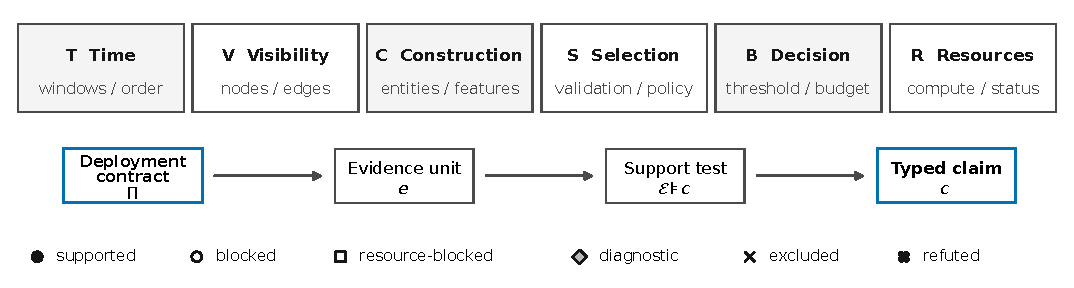
\includegraphics[width=0.90\textwidth]{fig01_deployment_contract.pdf}
    \caption{A deployment contract identifies the evidence unit and the support test applied to a typed claim. Status is an evidence outcome, not a color-coded performance rank.}
    \label{fig:s-contract-v2}
\end{figure}

\paragraph{Interpretive limit.}
Numerical equality across two contracts does not establish that their information access or estimands are interchangeable. Conversely, a numerical difference does not by itself identify which contract coordinate caused the change.

\section{Support-relation properties and controlled validation}
\label{sec:s-support}

\subsection{Properties}

The support relation treats benchmark reporting as a measurement problem: claims, operational interpretations, and evidence scopes are recorded together~\cite{jacobs2021measurement,reuel2024betterbench,bordes2025evalfacts}. Table~\ref{tab:s-support-properties} summarizes the five properties used by the validator.

\begin{table}[tbp]
\centering
\footnotesize
\setlength{\tabcolsep}{3.2pt}
\renewcommand{\arraystretch}{1.12}
\caption{Properties enforced by the typed support relation.}
\label{tab:s-support-properties}
\begin{tabularx}{\textwidth}{@{}l >{\raggedright\arraybackslash}p{0.25\textwidth} Y@{}}
\toprule
\textbf{ID} & \textbf{Property} & \textbf{Operational consequence} \\
\midrule
P1 & Scope monotonicity & Widening a claim adds requirements; it cannot erase requirements already named. \\
P2 & Evidence restriction & Removing the only admissible witness for a required element breaks support. \\
P3 & Rank invariance & Strictly increasing score calibration preserves AUROC/AUPRC ordering but may change a fixed-threshold decision. \\
P4 & Protocol non-substitutability & A result under one claim-relevant visibility or selection coordinate cannot fill another without an invariance argument. \\
P5 & Resource separation & A resource-blocked cell is measurable for feasibility but unordered by predictive performance. \\
\bottomrule
\end{tabularx}
\vspace{2pt}
\begin{minipage}{\textwidth}\footnotesize\emph{Scope and reading.} These are specification and ordering properties, not claims that the ontology is complete or that the validator establishes scientific truth.\end{minipage}
\end{table}


\begin{proposition}[Scope monotonicity of requirements]
If \(c'\) widens \(c\) by adding datasets, protocols, models, seeds, or resource regimes while holding the predicate fixed, then \(\Required(c)\subseteq\Required(c')\).
\end{proposition}
\begin{proof}[Proof sketch]
The requirement builder retains every named cell and auxiliary record and adds the widened scope. It never deletes an existing requirement. The property concerns requirements; it does not make truth monotone.
\end{proof}

\begin{proposition}[Evidence restriction]
If \(e\) is the only admissible witness for an element of \(\Required(c)\), then removing \(e\) breaks support for \(c\).
\end{proposition}
\begin{proof}
The required element becomes uncovered. Duplicate files with the same validated scientific key do not create a second independent witness.
\end{proof}

\begin{proposition}[Rank invariance under increasing calibration]
If \(g\) is strictly increasing and tie order is unchanged, replacing \(q_i\) with \(g(q_i)\) preserves AUROC and AUPRC but may change decisions at a fixed numerical threshold.
\end{proposition}
\begin{proof}
The rank metrics depend on score order, which \(g\) preserves. The selected set \(\{i:q_i\geq\tau\}\) need not equal \(\{i:g(q_i)\geq\tau\}\).
\end{proof}

\begin{proposition}[Protocol non-substitutability]
A result under \(\Pi_1\) cannot satisfy a requirement scoped to \(\Pi_2\) when the contracts differ on a claim-relevant coordinate, absent a separate invariance argument.
\end{proposition}
\begin{proof}[Proof sketch]
The contract is part of the scientific key. Changing a claim-relevant coordinate changes admissible information or the evaluation condition.
\end{proof}

\begin{proposition}[Resource separation]
A resource-blocked cell has no predictive ordering relation to a measured cell.
\end{proposition}
\begin{proof}
The blocked cell has no observed AUPRC, AUROC, or F1. It can be compared only as a feasibility outcome under \(\mathcal{R}\).
\end{proof}

\subsection{Controlled implementation validation}

Table~\ref{tab:s-validation-cases} reports the complete controlled suite. Each case starts from a frozen claim/evidence relation and changes one required property in a sandbox: scope, seed completeness, prediction presence, integrity, construct identity, resource state, or direction.

\begingroup
\footnotesize
\setlength{\tabcolsep}{3pt}
\renewcommand{\arraystretch}{1.10}
\begin{longtable}{@{}p{0.07\textwidth} p{0.18\textwidth} p{0.38\textwidth} p{0.15\textwidth} p{0.15\textwidth}@{}}
\caption{Controlled support-relation validation cases (14 of 14 matched the expected status).}\label{tab:s-validation-cases}\\
\toprule
\textbf{Case} & \textbf{Base claim} & \textbf{Controlled mutation} & \textbf{Expected} & \textbf{Observed} \\
\midrule
\endfirsthead
\caption[]{Controlled support-relation validation cases (14 of 14 matched the expected status). (continued)}\\
\toprule
\textbf{Case} & \textbf{Base claim} & \textbf{Controlled mutation} & \textbf{Expected} & \textbf{Observed} \\
\midrule
\endhead
\midrule
\multicolumn{5}{r}{\footnotesize Continued on next page}\\
\endfoot
\bottomrule
\endlastfoot
FV01 & C01 Elliptic visibility ranking & none; complete locked grid & \texttt{SUPPORTED} & \texttt{SUPPORTED} \\
FV02 & C01 Elliptic visibility ranking & remove one model/protocol cell in sandbox & \texttt{BLOCKED\_\allowbreak{}INCOMPLETE\_\allowbreak{}SCOPE} & \texttt{BLOCKED\_\allowbreak{}INCOMPLETE\_\allowbreak{}SCOPE} \\
FV03 & C01 Elliptic visibility ranking & remove seed 10 from one cell in sandbox & \texttt{BLOCKED\_\allowbreak{}INCOMPLETE\_\allowbreak{}SEEDS} & \texttt{BLOCKED\_\allowbreak{}INCOMPLETE\_\allowbreak{}SEEDS} \\
FV04 & C01 Elliptic visibility ranking & erase one prediction-manifest reference in sandbox & \texttt{BLOCKED\_\allowbreak{}MISSING\_\allowbreak{}PREDICTIONS} & \texttt{BLOCKED\_\allowbreak{}MISSING\_\allowbreak{}PREDICTIONS} \\
FV05 & C10 Small GINE AUPRC result & widen scope from Small to Medium & \texttt{RESOURCE\_\allowbreak{}BLOCKED} & \texttt{RESOURCE\_\allowbreak{}BLOCKED} \\
FV06 & C05 IBM AML baseline grid & widen scope from Small/Medium to all official variants & \texttt{RESOURCE\_\allowbreak{}BLOCKED} & \texttt{RESOURCE\_\allowbreak{}BLOCKED} \\
FV07 & V22 loss robustness & substitute a partial failed import for a full10 lane & \texttt{EXCLUDED\_\allowbreak{}INTEGRITY} & \texttt{EXCLUDED\_\allowbreak{}INTEGRITY} \\
FV08 & V24 temporal stress & treat three metadata labels as distinct temporal windows & \texttt{EXCLUDED\_\allowbreak{}CONSTRUCT\_\allowbreak{}INVALID} & \texttt{EXCLUDED\_\allowbreak{}CONSTRUCT\_\allowbreak{}INVALID} \\
FV09 & DGraphFin fixed GAT performance & promote the T4-OOM cell to a predictive comparison & \texttt{RESOURCE\_\allowbreak{}BLOCKED} & \texttt{RESOURCE\_\allowbreak{}BLOCKED} \\
FV10 & DGraphFin GraphSAGE max-pool rerun & promote runbook/status files without imported rows & \texttt{RESOURCE\_\allowbreak{}BLOCKED} & \texttt{RESOURCE\_\allowbreak{}BLOCKED} \\
FV11 & IBM sender-receiver construction & count the contract alias as an independent replication & \texttt{EXCLUDED\_\allowbreak{}CONSTRUCT\_\allowbreak{}INVALID} & \texttt{EXCLUDED\_\allowbreak{}CONSTRUCT\_\allowbreak{}INVALID} \\
FV12 & C04 universal graph harm & widen mixed scoped results into a universal directional claim & \texttt{REFUTED\_\allowbreak{}IN\_\allowbreak{}SCOPE} & \texttt{REFUTED\_\allowbreak{}IN\_\allowbreak{}SCOPE} \\
FV13 & C17 universal GraphSafe improvement & widen bounded mixed case study to universal dominance & \texttt{REFUTED\_\allowbreak{}IN\_\allowbreak{}SCOPE} & \texttt{REFUTED\_\allowbreak{}IN\_\allowbreak{}SCOPE} \\
FV14 & IBM early-to-late visibility & describe the shared first-60\% label-free node-history map as first-50\% training-only features & \texttt{EXCLUDED\_\allowbreak{}CONSTRUCT\_\allowbreak{}INVALID} & \texttt{EXCLUDED\_\allowbreak{}CONSTRUCT\_\allowbreak{}INVALID} \\
\end{longtable}
\noindent\footnotesize\emph{Scope and reading.} The cases localize incomplete scope, missing seeds or predictions, integrity and construct failures, resource blocks, and directional refutation. They are project-authored conformance tests, not external validation.\par
\endgroup


All 14 observed statuses equal their expected statuses. FV08 rejects the V24 stress-label interpretation because the label never reached the harness; FV11 rejects the sender-receiver alias as an independent method; FV14 rejects a first-50\%-only description of IBM account histories. These cases show that the implementation preserves the declared status distinctions.

\begin{figure}[tbp]
    \centering
    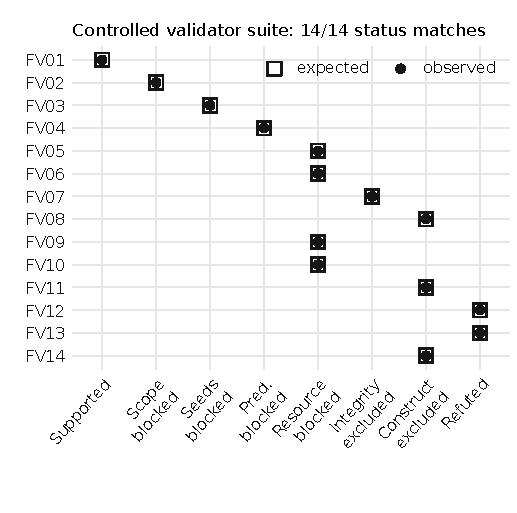
\includegraphics[width=0.86\textwidth]{fig08_claim_support_validation.pdf}
    \caption{Observed transitions for the 14 controlled claim/evidence mutations. The suite tests conformance to the project specification, not universal validator correctness.}
    \label{fig:s-support-validation-v2}
\end{figure}

\paragraph{What this does not establish.}
The schema, cases, and implementation were authored in the same project. Passing the suite does not prove ontology completeness, scientific truth, causal validity, curator agreement, fairness, or responsible deployment.

\section{Dataset cards}
\label{sec:s-datasets}

The three dataset families differ in prediction unit, label eligibility, graph semantics, temporal construction, prevalence, and empirical scope. They are therefore presented as separate cards rather than compressed into one cross-task leaderboard.

\subsection{Elliptic}

Elliptic is a real, pseudonymized Bitcoin transaction graph~\cite{weber2019aml}. Nodes are transactions with 165 features and 49 discrete time steps. The loader symmetrizes the 234,355 source edges to 468,710 message-passing arcs. Unknown transactions can contribute unlabeled context but are excluded from supervised denominators.

\begin{table}[tbp]
\centering
\footnotesize
\setlength{\tabcolsep}{3.2pt}
\renewcommand{\arraystretch}{1.12}
\caption{Elliptic dataset card.}
\label{tab:s-dataset-elliptic}
\begin{tabularx}{\textwidth}{@{}>{\raggedright\arraybackslash}p{0.23\textwidth} Y@{}}
\toprule
\textbf{Field} & \textbf{Verified value} \\
\midrule
Origin & real pseudonymized Bitcoin transactions \\
Prediction unit & transaction node \\
Graph size & 203,769 nodes; 234,355 source edges; 468,710 message-passing arcs \\
Features & 165 node; 0 edge \\
Temporal order & 49 discrete time steps \\
Protocols/windows & strict/isolated/transductive; train t1-30, val t31-34, test t35-49 \\
Train/validation/test & 26,905 / 2,989 / 16,670 eligible units \\
Positive counts & 2,954 / 508 / 1,083 \\
Test prevalence & 6.497\% \\
Label mapping & raw 1=illicit->positive 1; raw 2=licit->supervised 0 (repository code 2); unknown excluded \\
Source surface & \path{data/raw/elliptic_txs_*.csv; results/runs_rb09v3/runs.csv} \\
Known limitation & The 49 steps are dataset time bins; conclusions do not imply calendar-time or institution-level generalization. \\
\bottomrule
\end{tabularx}
\vspace{2pt}
\begin{minipage}{\textwidth}\footnotesize\emph{Scope and reading.} Counts and label mappings are recovered from the frozen dataset/task statistics. Unknown node labels remain graph context but never enter supervised masks.\end{minipage}
\end{table}


The card answers which units are scored and how the chronological masks are formed. It does not make the 49 bins equivalent to calendar time or establish behavior on another blockchain.

\subsection{DGraphFin}

DGraphFin is a real, anonymized financial-user graph~\cite{huang2022dgraph}. The task scores account nodes. Raw background classes 2 and 3 are mapped to unknown and excluded from supervised masks. Node time is the median timestamp of incident edges, followed by 20 equal-count buckets; isolated nodes receive the global median timestamp.

\begin{table}[tbp]
\centering
\footnotesize
\setlength{\tabcolsep}{3.2pt}
\renewcommand{\arraystretch}{1.12}
\caption{DGraphFin dataset card.}
\label{tab:s-dataset-dgraphfin}
\begin{tabularx}{\textwidth}{@{}>{\raggedright\arraybackslash}p{0.23\textwidth} Y@{}}
\toprule
\textbf{Field} & \textbf{Verified value} \\
\midrule
Origin & real anonymized financial user graph \\
Prediction unit & account/user node \\
Graph size & 3,700,550 nodes; 4,300,999 source edges; 7,994,520 message-passing arcs \\
Features & 17 node; 0 edge \\
Temporal order & 20 equal-count incident-edge timestamp buckets \\
Protocols/windows & strict/isolated/transductive; train t1-14, val t15-16, test t17-20 \\
Train/validation/test & 947,462 / 107,932 / 170,207 eligible units \\
Positive counts & 12,543 / 1,103 / 1,863 \\
Test prevalence & 1.095\% \\
Label mapping & raw 1=fraud->positive 1; raw 0=normal->supervised 0 (repository code 2); raw 2/3 background excluded \\
Source surface & \path{data/raw/dgraphfin.npz; results/runs_rb09v3/runs.csv} \\
Known limitation & Time is a median incident-edge timestamp placed into equal-count buckets, not a calendar deployment schedule. \\
\bottomrule
\end{tabularx}
\vspace{2pt}
\begin{minipage}{\textwidth}\footnotesize\emph{Scope and reading.} Counts and label mappings are recovered from the frozen dataset/task statistics. Unknown node labels remain graph context but never enter supervised masks.\end{minipage}
\end{table}


The equal-count bucket construction is an implementation choice. It supports the reported fixed split but not a claim about a particular calendar horizon or bank workflow.

\subsection{IBM AML-Data}

IBM AML-Data is synthetic financial-transaction data, not bank production evidence~\cite{altman2023ibmaml}. The task scores directed transaction edges in HI/LI Small/Medium account networks. HI and LI identify generation regimes with different laundering frequencies; they are not severity labels.

\begin{table}[tbp]
\centering
\footnotesize
\setlength{\tabcolsep}{3.2pt}
\renewcommand{\arraystretch}{1.12}
\caption{IBM AML-Data dataset card.}
\label{tab:s-dataset-ibm}
\begin{tabularx}{\textwidth}{@{}>{\raggedright\arraybackslash}p{0.23\textwidth} Y@{}}
\toprule
\textbf{Field} & \textbf{Verified value} \\
\midrule
Origin & Synthetic financial transactions from IBM AML-Data \\
Prediction unit & Directed transaction edge \\
Measured variants & HI MEDIUM, HI SMALL, LI MEDIUM, LI SMALL \\
Graph range & 515,088--2,077,023 accounts; 5,078,345--31,898,238 transactions \\
Features & Eight transaction attributes and eight account-history attributes \\
Temporal order & Stable chronological transaction sort \\
Labels & is\_laundering=1 positive; 0 negative; no unknown class in the materialized task \\
Visibility & Classifier labels use 50\% or 60\% by protocol; both protocols share the first-60\% label-free account-history map \\
Unmeasured scope & HI/LI Large are guard-blocked; HI/LI Medium GINE h64 is T4-OOM \\
Known limitation & HI/LI are synthetic generator regimes, not observed bank populations or severity categories \\
\bottomrule
\end{tabularx}
\vspace{2pt}
\begin{minipage}{\textwidth}\footnotesize\emph{Scope and reading.} Predictive evidence exists only for the four Small/Medium variants. Large and Medium-GINE cells are retained as resource outcomes, not assigned performance.\end{minipage}
\end{table}


The measured graphs range from roughly 5.1 million to 31.9 million transaction edges. Their scale is useful for resource and construction analysis, but one synthetic generator does not establish representativeness across institutions, typologies, jurisdictions, or adversarial adaptation.

\paragraph{Cross-dataset interpretation.}
Elliptic transaction nodes, DGraphFin account nodes, and IBM transaction edges answer different questions. Their raw AUPRC values, prevalences, and feasible models are retained within typed evidence units and never averaged into a universal score.

\section{Temporal windows and visibility matrices}
\label{sec:s-visibility}

\subsection{Node-task contracts}

Strict-inductive and isolated-inductive use identical temporal masks and training subgraphs. During evaluation, strict-inductive exposes the held-out structure with labels hidden. Isolated-inductive removes every edge with exactly one endpoint in the held-out union, so held-out nodes can communicate among themselves but not across the train/held-out boundary. The transductive comparator exposes the full graph during training and evaluation while withholding validation/test labels from the loss.

Table~\ref{tab:s-protocol-cards} separates these access choices from selection and decision rules.

\begin{table}[tbp]
\centering
\footnotesize
\setlength{\tabcolsep}{3.2pt}
\renewcommand{\arraystretch}{1.12}
\caption{Protocol cards keep time, visibility, selection, and decision coordinates separate.}
\label{tab:s-protocol-cards}
\begin{tabularx}{\textwidth}{@{}>{\raggedright\arraybackslash}p{0.12\textwidth} >{\raggedright\arraybackslash}p{0.13\textwidth} Y Y Y >{\raggedright\arraybackslash}p{0.12\textwidth}@{}}
\toprule
\textbf{Protocol} & \textbf{Masks} & \textbf{Graph/covariate visibility} & \textbf{Labels} & \textbf{Selection/decision} & \textbf{Datasets} \\
\midrule
Strict & chronological & training nodes/edges only during training; held-out structure available at evaluation & test labels hidden & validation F1 & Elliptic, DGraphFin \\
Isolated & same chronological masks & held-out nodes isolated from training-period cross-split edges at evaluation & test labels hidden & validation F1 & Elliptic, DGraphFin \\
Transductive & same masks & full graph structure visible & test labels hidden & validation F1 & Elliptic, DGraphFin \\
Late-window & 60/20/20 chronological & shared node-history map uses first 60\%, which is this protocol's training interval & test transaction labels hidden & fixed 0.5 threshold for saved F1 & IBM AML-Data \\
Early-to-late & 50/20/30 chronological & classifier labels use first 50\%; shared label-free node-history map uses first 60\%, including covariates from 50-60\% & test transaction labels hidden & fixed 0.5 threshold for saved F1 & IBM AML-Data \\
\bottomrule
\end{tabularx}
\vspace{2pt}
\begin{minipage}{\textwidth}\footnotesize\emph{Scope and reading.} Strict and isolated protocols share masks but differ in graph access. IBM early-to-late is explicitly a 50\% labeled-training / 60\% label-free-history contract.\end{minipage}
\end{table}


The key interpretation is visibility sensitivity under fixed masks, not a causal decomposition of homophily, degree shift, oversmoothing, or temporal mechanisms.

\subsection{Access matrix}

Table~\ref{tab:s-visibility-matrix} states labeled access, validation use, test-feature access, graph access, historical covariates, selection/threshold, and resource scope independently.

\begingroup
\footnotesize
\setlength{\tabcolsep}{3pt}
\renewcommand{\arraystretch}{1.10}
\begin{longtable}{@{}p{0.11\textwidth} p{0.10\textwidth} p{0.09\textwidth} p{0.06\textwidth} p{0.18\textwidth} p{0.15\textwidth} p{0.11\textwidth} p{0.10\textwidth}@{}}
\caption{Access matrix for the five evaluated deployment contracts.}\label{tab:s-visibility-matrix}\\
\toprule
\textbf{Contract} & \textbf{Labeled train} & \textbf{Validation} & \textbf{Test features} & \textbf{Graph nodes/edges} & \textbf{Historical covariates} & \textbf{Decision rule} & \textbf{Resources} \\
\midrule
\endfirsthead
\caption[]{Access matrix for the five evaluated deployment contracts. (continued)}\\
\toprule
\textbf{Contract} & \textbf{Labeled train} & \textbf{Validation} & \textbf{Test features} & \textbf{Graph nodes/edges} & \textbf{Historical covariates} & \textbf{Decision rule} & \textbf{Resources} \\
\midrule
\endhead
\midrule
\multicolumn{8}{r}{\footnotesize Continued on next page}\\
\endfoot
\bottomrule
\endlastfoot
Strict & Chronological train & Validation F1 & Yes & Held-out structure at evaluation & Training-period only & Validation-selected & Recorded run envelope \\
Isolated & Same train & Validation F1 & Yes & Held-out subgraph; no train/held-out cross edges & Training-period only & Validation-selected & Recorded run envelope \\
Transductive & Same train & Validation F1 & Yes & Full graph during training/evaluation; held-out labels hidden & Full visible graph & Validation-selected & Recorded run envelope \\
IBM late-window & First 60\% labels & Next 20\% & Yes & Account graph and transaction features & First 60\% label-free history & Fixed 0.5 F1 threshold & Small/Medium measured \\
IBM early-to-late & First 50\% labels & Next 20\% & Yes & Account graph and transaction features & Shared first 60\%; includes 50--60\% label-free covariates & Fixed 0.5 F1 threshold & Small/Medium measured \\
\end{longtable}
\noindent\footnotesize\emph{Scope and reading.} Test labels are hidden in every evaluation. Access to test features or graph structure is a declared contract coordinate and must not be confused with access to test labels.\par
\endgroup


Test labels are never exposed. Test features or structure may be visible when the declared deployment contract permits them. Calling all non-label access \emph{leakage} would collapse scientifically different contracts; failing to disclose it would be equally misleading.

\subsection{IBM temporal windows}

IBM late-window uses 60/20/20 chronological masks. Early-to-late uses 50/20/30 classifier masks, but both protocols reuse an account-history matrix constructed from the first 60\% of transactions. Thus early-to-late receives label-free covariates from 50--60\%, half of its nominal validation interval.

\begingroup
\footnotesize
\setlength{\tabcolsep}{3pt}
\renewcommand{\arraystretch}{1.10}
\begin{longtable}{@{}p{0.12\textwidth} p{0.14\textwidth} r r r r r@{}}
\caption{Exact IBM temporal-window counts and test prevalence.}\label{tab:s-ibm-windows}\\
\toprule
\textbf{Variant} & \textbf{Protocol} & \textbf{Train} & \textbf{Validation} & \textbf{Test} & \textbf{Test positives} & \textbf{Test prevalence} \\
\midrule
\endfirsthead
\caption[]{Exact IBM temporal-window counts and test prevalence. (continued)}\\
\toprule
\textbf{Variant} & \textbf{Protocol} & \textbf{Train} & \textbf{Validation} & \textbf{Test} & \textbf{Test positives} & \textbf{Test prevalence} \\
\midrule
\endhead
\midrule
\multicolumn{7}{r}{\footnotesize Continued on next page}\\
\endfoot
\bottomrule
\endlastfoot
HI MEDIUM & Early-to-late & 15,949,119 & 6,379,647 & 9,569,472 & 14,147 & 0.148\% \\
HI MEDIUM & Late-window & 19,138,942 & 6,379,648 & 6,379,648 & 10,642 & 0.167\% \\
HI SMALL & Early-to-late & 2,539,172 & 1,015,669 & 1,523,504 & 2,321 & 0.152\% \\
HI SMALL & Late-window & 3,047,007 & 1,015,669 & 1,015,669 & 1,797 & 0.177\% \\
LI MEDIUM & Early-to-late & 15,625,741 & 6,250,297 & 9,375,445 & 5,392 & 0.058\% \\
LI MEDIUM & Late-window & 18,750,889 & 6,250,297 & 6,250,297 & 3,783 & 0.061\% \\
LI SMALL & Early-to-late & 3,462,024 & 1,384,810 & 2,077,215 & 1,334 & 0.064\% \\
LI SMALL & Late-window & 4,154,429 & 1,384,810 & 1,384,810 & 925 & 0.067\% \\
\end{longtable}
\noindent\footnotesize\emph{Scope and reading.} The table reports prediction-unit denominators. It does not pool HI/LI or Small/Medium, and the early-to-late history visibility remains the shared first-60\% map described above.\par
\endgroup


The exact denominators and prevalences explain why raw values remain context-specific. The shared 60\% history is not test-label leakage, yet it prevents a pure first-50\%-only information claim and blocks causal attribution of protocol differences to label-window timing alone.

\section{Graph-construction definitions}
\label{sec:s-constructions}

The IBM construction study uses the edge-aware SAGE-derived h64 classifier as its reference. Every intervention retains variant, protocol, seed, and optimizer schedule unless the intervention itself changes the training structure. Table~\ref{tab:s-construction-cards} records the operation and question for each matched candidate.

\begin{table}[tbp]
\centering
\footnotesize
\setlength{\tabcolsep}{3.2pt}
\renewcommand{\arraystretch}{1.12}
\caption{Matched IBM graph-construction and feature interventions.}
\label{tab:s-construction-cards}
\begin{tabularx}{\textwidth}{@{}>{\raggedright\arraybackslash}p{0.16\textwidth} Y Y >{\raggedright\arraybackslash}p{0.20\textwidth}@{}}
\toprule
\textbf{Construction} & \textbf{Operation} & \textbf{Question} & \textbf{Matched scope} \\
\midrule
NoEdge & zero transaction attributes; structure retained & tests edge-attribute contribution & matched to h64 reference \\
ShuffledEdge & edge attributes permuted within temporal masks & destroys edge-feature alignment while preserving marginal values & matched to h64 reference \\
DegreeOnly & endpoint-degree attributes replace transaction features & tests structural summaries without original attributes & matched to h64 reference \\
DegreeCap & q=.995 cap on training structure & tests hub sensitivity and resource/performance tradeoff & matched to h64 reference \\
RecentWindow & most recent 50\% of training edges & tests recency and reduced computation & matched to h64 reference \\
Sender-receiver alias & Restates the already materialized sender-to-receiver transaction edges & Contract identity check; no new transformation & Diagnostic only; never counted as an independent method \\
\bottomrule
\end{tabularx}
\vspace{2pt}
\begin{minipage}{\textwidth}\footnotesize\emph{Scope and reading.} Every intervention retains variant, protocol, seed, optimizer schedule, and h64 reference family unless the operation itself changes training structure. The sender-receiver row is an alias, not replication.\end{minipage}
\end{table}


\paragraph{Feature controls.}
NoEdge sets all eight transaction attributes to zero while preserving account structure and histories. ShuffledEdge permutes transaction-feature rows separately within train, validation, and test masks, preserving marginal distributions and split sizes while breaking transaction-to-feature alignment. DegreeOnly replaces the transaction attributes with source/destination in/out-degree summaries computed from training edges.

\paragraph{Structural controls.}
DegreeCap removes training edges incident to accounts above the 0.995 active-training-degree quantile, subject to safety guards. RecentWindow uses only the chronologically latest 50\% of training edges to construct the training structure, changing both represented history and computation.

\paragraph{Identity diagnostic.}
The sender-receiver row records that the materialized arrays already encode sender-to-receiver transactions. It performs no independent graph transformation. Its matched zero rows remain useful as an identity check but cannot count as replication or as another method in a winner set.

\paragraph{Interpretive limit.}
These interventions isolate implementation-level representation and construction choices within the recorded IBM contracts. They do not identify causal effects for arbitrary AML networks, and Medium GINE remains outside the feasible set.

\section{Model cards and equations}
\label{sec:s-models-v2}

\subsection{Node classifiers}

The feature-only MLP does not consume adjacency and therefore serves as a negative control for the graph-only visibility intervention. The GCN update is
\begin{equation}
 H^{(\ell+1)}
 =\sigma\!\left(\widehat D^{-1/2}\widehat A\widehat D^{-1/2}
 H^{(\ell)}W^{(\ell)}\right),
\end{equation}
with self-loops in \(\widehat A\)~\cite{kipf2017gcn}. Mean GraphSAGE uses
\begin{equation}
 h_v^{(\ell+1)}
 =\sigma\!\left(W^{(\ell)}
 [h_v^{(\ell)}\Vert |N(v)|^{-1}\!\sum_{u\in N(v)}h_u^{(\ell)}]\right)
\end{equation}
and therefore depends differently on available neighborhoods~\cite{hamilton2017graphsage}.

\begin{table}[tbp]
\centering
\footnotesize
\setlength{\tabcolsep}{3.2pt}
\renewcommand{\arraystretch}{1.12}
\caption{Node-classifier cards for Elliptic and DGraphFin.}
\label{tab:s-node-models}
\begin{tabularx}{\textwidth}{@{}>{\raggedright\arraybackslash}p{0.16\textwidth} Y Y >{\raggedright\arraybackslash}p{0.22\textwidth}@{}}
\toprule
\textbf{Model} & \textbf{Computation} & \textbf{Scientific role} & \textbf{Configuration} \\
\midrule
MLP & node features only & negative control for graph-visibility intervention & Elliptic h256/l3; DGraphFin h64/l2 \\
GCN & normalized neighborhood aggregation & tests spectral-style smoothing under visibility change & Elliptic h256/l3; DGraphFin h64/l2 \\
GraphSAGE & mean neighborhood aggregation & tests inductive aggregation under visibility change & Elliptic h256/l3; DGraphFin h64/l2 \\
\bottomrule
\end{tabularx}
\vspace{2pt}
\begin{minipage}{\textwidth}\footnotesize\emph{Scope and reading.} The MLP is the graph-visibility negative control. The grid does not establish class-wide behavior for modern temporal or heterogeneous GNNs.\end{minipage}
\end{table}


The card makes the architecture control explicit: Elliptic uses h256/l3 while DGraphFin uses h64/l2. The grid studies three mostly static families and does not support a class-wide conclusion about temporal-state, transformer, or heterogeneous GNNs.

\subsection{IBM transaction classifiers}

Logistic regression and histogram gradient boosting operate on transaction attributes without account-graph message passing~\cite{friedman2001gbm}. The SAGE-derived edge classifiers first form one-hop training-history summaries
\begin{equation}
 \bar x_{N(v)}
 =\frac{1}{\max(1,|N_{\mathrm{tr}}(v)|)}
 \sum_{u\in N_{\mathrm{tr}}(v)}x_u,
 \qquad
 \widetilde x_v=[x_v\Vert\bar x_{N(v)}],
\end{equation}
then score transaction \((u,v)\) with
\begin{equation}
 q_{uv}=\sigma\!\left(f_\theta(
 [\widetilde x_u\Vert\widetilde x_v\Vert a_{uv}])\right).
\end{equation}
They are static one-hop edge classifiers, not stacks of sampled GraphSAGE convolutions.

The feasible GINE candidate uses one edge-conditioned update,
\begin{equation}
 h_v'=\operatorname{MLP}\!\left((1+\epsilon)h_v+
 \sum_{u\in N(v)}\operatorname{ReLU}(h_u+\phi(a_{uv}))\right),
\end{equation}
followed by an edge head~\cite{hu2020pretraining}.

\begin{table}[tbp]
\centering
\footnotesize
\setlength{\tabcolsep}{3.2pt}
\renewcommand{\arraystretch}{1.12}
\caption{IBM transaction-classifier cards.}
\label{tab:s-ibm-models}
\begin{tabularx}{\textwidth}{@{}>{\raggedright\arraybackslash}p{0.20\textwidth} Y Y >{\raggedright\arraybackslash}p{0.20\textwidth}@{}}
\toprule
\textbf{Model} & \textbf{Input/computation} & \textbf{Scientific role} & \textbf{Configuration} \\
\midrule
Logistic regression & standardized transaction features & linear non-graph baseline & balanced classes; max\_iter=500 \\
Histogram gradient boosting & transaction features & nonlinear tabular baseline & 160 iterations; learning rate 0.06 \\
GraphSAGE-derived edge classifier h32 & training-history endpoint/neighborhood summaries plus edge features & small IBM graph baseline & 20 epochs; batch 65,536 \\
Edge-aware GraphSAGE-derived edge classifier h64 & training-history endpoint/neighborhood summaries plus edge features & reference for graph-feature/construction ablations & 30 epochs; batch 32,768 \\
GINE h64 & one GINE layer and edge head & edge-conditioned message-passing architecture & 30 epochs; batch 32,768; Small only \\
\bottomrule
\end{tabularx}
\vspace{2pt}
\begin{minipage}{\textwidth}\footnotesize\emph{Scope and reading.} The h32/h64 systems are static one-hop GraphSAGE-derived edge classifiers. Medium GINE is resource-blocked and has no performance value.\end{minipage}
\end{table}


GINE h64 is measured only on Small. The two Medium lanes exhausted a T4 and receive no performance score. The model card preserves that feasibility condition alongside the computational definition.

\section{Optimization, selection, and thresholding}
\label{sec:s-optimization}

Table~\ref{tab:s-training-cards} consolidates optimizer, learning rate, regularization, loss, schedule, validation selection, threshold, and batching. These choices are scientific coordinates because changing selection or threshold can change a decision-level conclusion even when score rankings are fixed.

\begingroup
\footnotesize
\setlength{\tabcolsep}{3pt}
\renewcommand{\arraystretch}{1.10}
\begin{longtable}{@{}p{0.14\textwidth} p{0.10\textwidth} p{0.07\textwidth} p{0.07\textwidth} p{0.12\textwidth} p{0.09\textwidth} p{0.13\textwidth} p{0.13\textwidth}@{}}
\caption{Optimization, validation selection, and decision settings.}\label{tab:s-training-cards}\\
\toprule
\textbf{Family} & \textbf{Optimizer} & \textbf{LR} & \textbf{Weight decay} & \textbf{Loss} & \textbf{Iterations} & \textbf{Selection} & \textbf{Decision/batch} \\
\midrule
\endfirsthead
\caption[]{Optimization, validation selection, and decision settings. (continued)}\\
\toprule
\textbf{Family} & \textbf{Optimizer} & \textbf{LR} & \textbf{Weight decay} & \textbf{Loss} & \textbf{Iterations} & \textbf{Selection} & \textbf{Decision/batch} \\
\midrule
\endhead
\midrule
\multicolumn{8}{r}{\footnotesize Continued on next page}\\
\endfoot
\bottomrule
\endlastfoot
Elliptic protocol grid & AdamW & 1e-3 & 5e-4 & class-weighted CE & 200 & validation F1 & argmax over 3 repository label codes; full graph forward \\
DGraphFin protocol grid & AdamW & 1e-3 & 5e-4 & class-weighted CE & 200 & validation F1 & argmax over 3 repository label codes; full graph forward \\
IBM LR & LBFGS family (scikit-learn) & library default & library default & balanced class weight & max\_iter 500 & training only & score >= .5; CPU \\
IBM HistGB & histogram gradient boosting & .06 & n/a & binary log loss & 160 & training only & score >= .5; CPU \\
IBM GraphSAGE-derived h32 & AdamW & 1e-3 & 1e-4 & positive-weighted BCE & 20 & fixed seed & score >= .5; edge minibatches 65,536 \\
IBM h64 graph grid & AdamW & 1e-3 & 1e-4 & positive-weighted BCE & 30 & fixed seed & score >= .5; edge minibatches 32,768 \\
\end{longtable}
\noindent\footnotesize\emph{Scope and reading.} Node-grid checkpoints are selected by validation F1. IBM saved F1 uses 0.5. Deterministic library baselines may repeat exactly across nominal seeds; those repetitions are not reinterpreted as independent stochastic fits.\par
\endgroup


\subsection{Node-grid selection}

Elliptic and DGraphFin use AdamW, class-weighted cross-entropy, cosine learning-rate decay, and a 200-epoch cap. Validation F1 is checked at epoch 1 and every ten epochs. Configured patience is 40 validation checks, so it cannot fire within the cap; the saved row is the best scheduled validation checkpoint. Python, NumPy, and PyTorch seeds are fixed per run, and features are standardized on training rows.

\subsection{IBM fitting and decisions}

The IBM tree and logistic baselines run on CPU. The h32 and h64 graph-derived classifiers use positive-weighted binary cross-entropy and edge minibatches. Saved IBM F1 uses threshold 0.5. No later threshold search is retroactively applied to those rows. Runtime records report the actual backend; a legacy path token containing P100 is not hardware evidence and is normalized to the recorded T4/CUDA lane.

\subsection{Deterministic baselines}

Some library baselines repeat exactly across nominal seeds. Their ten rows document repeated pipeline evaluation and confirm deterministic output under the saved configuration, but they are not reinterpreted as ten independent stochastic fits. Zero variance remains visible in the aggregate intervals.

\paragraph{Interpretive limit.}
The settings reproduce the saved evidence surface. They do not establish that the hyperparameter grid is exhaustive or optimal for another institution, time period, hardware stack, or model implementation.

\section{Metrics and statistical procedure}
\label{sec:s-statistics-v2}

\subsection{Estimands}

AUPRC is the primary ranking metric under severe imbalance because ROC curves can obscure low precision~\cite{saito2015pr}. AUROC, fixed-threshold F1, review-budget precision/recall, calibration, and illustrative cost answer different questions. Table~\ref{tab:s-metric-cards} states each estimand and its boundary.

\begin{table}[tbp]
\centering
\footnotesize
\setlength{\tabcolsep}{3.2pt}
\renewcommand{\arraystretch}{1.12}
\caption{Metric cards distinguish ranking, decision, capacity, and calibration questions.}
\label{tab:s-metric-cards}
\begin{tabularx}{\textwidth}{@{}>{\raggedright\arraybackslash}p{0.16\textwidth} >{\raggedright\arraybackslash}p{0.12\textwidth} Y Y@{}}
\toprule
\textbf{Metric} & \textbf{Type} & \textbf{Estimand} & \textbf{Interpretation boundary} \\
\midrule
AUPRC & Rank & Area under precision-recall curve & Primary rare-event ranking metric; interpreted against within-cell prevalence. \\
AUROC & Rank & Probability a random positive outranks a random negative & Can remain high when precision is poor under severe imbalance. \\
F1@0.5 & Decision & Harmonic mean of precision and recall & IBM operating point only; not threshold-invariant. \\
Precision/Recall@b & Capacity & Top K scores where K is the declared review fraction & Reported at 0.5\%, 1\%, and 2\%; queue-capacity conditioned. \\
Normalized AUPRC & Diagnostic & AUPRC divided by test prevalence & Lift context only; not a prevalence-invariant universal metric. \\
Brier score & Calibration & Mean squared probability error & Descriptive on saved predictions; lower is better. \\
ECE & Calibration & Ten-bin expected calibration error & Binning dependent and descriptive. \\
Cost risk & Decision & FP + 5 FN divided by evaluation size & Illustrative 1:5 scenario, not bank monetary loss. \\
\bottomrule
\end{tabularx}
\vspace{2pt}
\begin{minipage}{\textwidth}\footnotesize\emph{Scope and reading.} No metric substitutes for another. In particular, monotone calibration cannot repair an AUPRC ranking, and fixed-threshold F1 cannot stand in for every review policy.\end{minipage}
\end{table}


At review fraction \(b\), \(K=\lceil b|I|\rceil\) and the top \(K\) scores form the queue. The cost scenario is
\begin{equation}
 R_c(\tau)=\frac{FP(\tau)+5FN(\tau)}{|I|},
\end{equation}
which is a 1:5 illustration rather than an estimate of bank loss~\cite{bahnsen2015cost}. Calibration is summarized by Brier score and ten-bin ECE; ECE remains binning-dependent~\cite{guo2017calibration}.

\subsection{Paired uncertainty and correction}

Primary cells use seeds 1--10. Arithmetic means and sample standard deviations describe the saved rows. Confidence intervals use 10,000 deterministic percentile-bootstrap resamples with random seed 20260710~\cite{efron1979bootstrap}. Paired effects match seed \(s\) on each side, and
\begin{equation}
 d_z=\frac{\overline{\Delta}}{s_\Delta}.
\end{equation}
Two-sided Wilcoxon signed-rank tests operate on nonzero paired differences; all-zero contrasts receive \(p=1\). Holm correction is applied within the declared primary families~\cite{holm1979}. The older V22 robustness table retains its existing Benjamini-Hochberg values and is not mixed into the new families~\cite{benjamini1995}.

\begin{table}[tbp]
\centering
\footnotesize
\setlength{\tabcolsep}{3.2pt}
\renewcommand{\arraystretch}{1.12}
\caption{Statistical families and inferential units.}
\label{tab:s-statistical-families}
\begin{tabularx}{\textwidth}{@{}>{\raggedright\arraybackslash}p{0.16\textwidth} >{\raggedright\arraybackslash}p{0.18\textwidth} Y Y >{\raggedright\arraybackslash}p{0.18\textwidth}@{}}
\toprule
\textbf{Family} & \textbf{Scope} & \textbf{Independent unit} & \textbf{Interval/test} & \textbf{Correction} \\
\midrule
Node visibility & 18 dataset-model-metric effects & 10 paired seeds & 10,000-resample percentile CI; paired dz; Wilcoxon & Holm within metric \\
IBM construction & Candidate vs h64 by size and metric & 10 seed blocks after averaging four fixed contexts within seed & 10,000-resample percentile CI; paired dz; Wilcoxon & Holm within size-by-metric \\
IBM context sensitivity & 208 context-specific effects & 10 paired seeds per fixed context & Descriptive CI, dz, and Wilcoxon & Context table is sensitivity, not a second confirmatory family \\
GraphSafe & 48 declared comparator-metric tests & 10 seed blocks after averaging six contexts within seed & Percentile CI and Wilcoxon & One Holm family of 48 \\
V22 robustness & 198 legacy paired tests & 10 paired seeds & Bootstrap CI and paired test & Original Benjamini-Hochberg values retained \\
\bottomrule
\end{tabularx}
\vspace{2pt}
\begin{minipage}{\textwidth}\footnotesize\emph{Scope and reading.} Ten seeds quantify optimization variation on fixed datasets and splits. They do not estimate population variation across banks, institutions, or future periods.\end{minipage}
\end{table}


For IBM construction effects, the four fixed HI/LI-by-protocol context differences are averaged within seed before inference, yielding ten seed blocks rather than 40 exchangeable pairs. GraphSafe similarly averages six contexts within seed before its ten-pair analysis. The statistical-family table makes these independent units explicit.

\paragraph{What the intervals do not establish.}
Ten seeds quantify optimization variation on fixed datasets and splits. Resampling does not create institution-level or future-period observations. A confidence interval excluding zero does not override a nonsignificant family-adjusted test, and resource-blocked cells remain absent rather than imputed.

\section{Elliptic and DGraphFin protocol results}
\label{sec:s-protocol-results}

\subsection{Scientific question and matched scope}

The primary question is whether changing only strict-versus-isolated graph visibility leaves each architecture invariant. Both sides use the same dataset, temporal masks, model configuration, and seeds. Tables~\ref{tab:s-protocol-auprc}--\ref{tab:s-protocol-f1} report all 18 aggregate effects; the complete 180 seed rows remain in the artifact.

\subsection{AUPRC}

\begin{table}[tbp]
\centering
\footnotesize
\setlength{\tabcolsep}{3.2pt}
\renewcommand{\arraystretch}{1.12}
\caption{Strict-to-isolated paired AUPRC effects.}
\label{tab:s-protocol-auprc}
\begin{tabularx}{\textwidth}{@{}>{\raggedright\arraybackslash}p{0.13\textwidth} >{\raggedright\arraybackslash}p{0.13\textwidth} r r r >{\raggedright\arraybackslash}p{0.21\textwidth} r r@{}}
\toprule
\textbf{Dataset} & \textbf{Model} & \textbf{n} & \textbf{Strict} & \textbf{Isolated} & \textbf{$\Delta$ [95\% CI]} & \textbf{$d_z$} & \textbf{Holm p} \\
\midrule
DGraphFin & GCN & 10 & 0.01164 & 0.01183 & +0.00019 [-0.00134, 0.00191] & 0.069 & 1.0000 \\
DGraphFin & MLP & 10 & 0.01398 & 0.01398 & +0.00000 [0.00000, 0.00000] & 0.000 & 1.0000 \\
DGraphFin & GraphSAGE & 10 & 0.02270 & 0.01781 & -0.00489 [-0.00640, -0.00331] & -1.877 & 0.0156 \\
Elliptic & GCN & 10 & 0.46664 & 0.56046 & +0.09382 [0.07898, 0.10818] & 3.765 & 0.0117 \\
Elliptic & MLP & 10 & 0.45216 & 0.45216 & +0.00000 [0.00000, 0.00000] & 0.000 & 1.0000 \\
Elliptic & GraphSAGE & 10 & 0.61139 & 0.47969 & -0.13170 [-0.14221, -0.12114] & -7.397 & 0.0117 \\
\bottomrule
\end{tabularx}
\vspace{2pt}
\begin{minipage}{\textwidth}\footnotesize\emph{Scope and reading.} All comparisons share seeds 1--10 and identical temporal masks. The intervention changes graph visibility; it does not identify a unique mechanism for the observed response.\end{minipage}
\end{table}


The MLP delta is exactly zero on both datasets, as expected for a graph-only intervention. On Elliptic, GraphSAGE changes from 0.61139 to 0.47969 (\(\Delta=-0.13170\)), while GCN changes from 0.46664 to 0.56046 (\(\Delta=0.09382\)); both Holm values are 0.0117. The leading model among MLP, GCN, and GraphSAGE therefore changes from GraphSAGE under strict visibility to GCN under isolated visibility. DGraphFin GraphSAGE declines from 0.02270 to 0.01781 (\(\Delta=-0.00489\), Holm \(p=0.0156\)), but remains the top model in the tested set.

\begin{figure}[tbp]
    \centering
    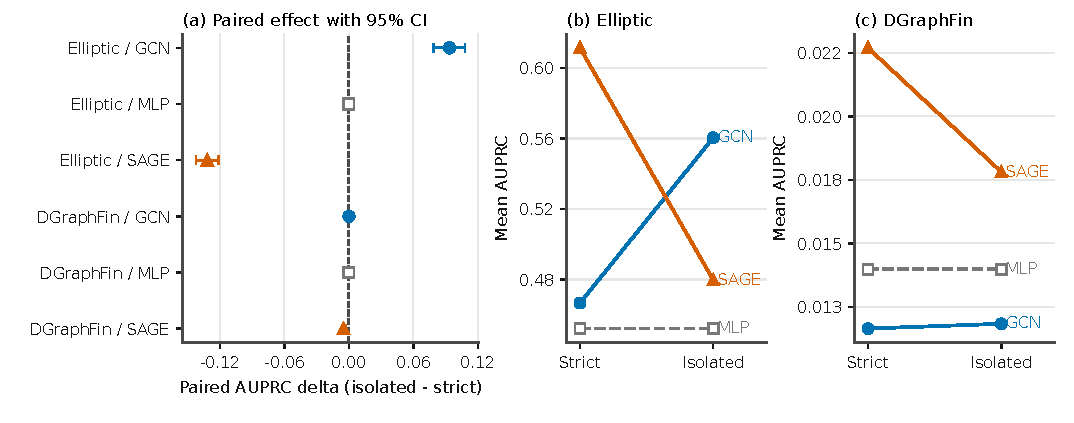
\includegraphics[width=0.86\textwidth]{fig02_protocol_architecture_effects.pdf}
    \caption{Paired strict-to-isolated AUPRC effects. The feature-only control remains invariant while graph-model direction and magnitude depend on architecture and dataset.}
    \label{fig:s-protocol-effects-v2}
\end{figure}

\subsection{AUROC}

\begin{table}[tbp]
\centering
\footnotesize
\setlength{\tabcolsep}{3.2pt}
\renewcommand{\arraystretch}{1.12}
\caption{Strict-to-isolated paired AUROC effects.}
\label{tab:s-protocol-auroc}
\begin{tabularx}{\textwidth}{@{}>{\raggedright\arraybackslash}p{0.13\textwidth} >{\raggedright\arraybackslash}p{0.13\textwidth} r r r >{\raggedright\arraybackslash}p{0.21\textwidth} r r@{}}
\toprule
\textbf{Dataset} & \textbf{Model} & \textbf{n} & \textbf{Strict} & \textbf{Isolated} & \textbf{$\Delta$ [95\% CI]} & \textbf{$d_z$} & \textbf{Holm p} \\
\midrule
DGraphFin & GCN & 10 & 0.53049 & 0.52091 & -0.00958 [-0.05269, 0.03227] & -0.131 & 1.0000 \\
DGraphFin & MLP & 10 & 0.52554 & 0.52554 & +0.00000 [0.00000, 0.00000] & 0.000 & 1.0000 \\
DGraphFin & GraphSAGE & 10 & 0.68688 & 0.65789 & -0.02899 [-0.03921, -0.01956] & -1.748 & 0.0117 \\
Elliptic & GCN & 10 & 0.87228 & 0.87002 & -0.00226 [-0.00769, 0.00195] & -0.270 & 1.0000 \\
Elliptic & MLP & 10 & 0.87458 & 0.87458 & +0.00000 [0.00000, 0.00000] & 0.000 & 1.0000 \\
Elliptic & GraphSAGE & 10 & 0.88744 & 0.86737 & -0.02007 [-0.02172, -0.01816] & -6.602 & 0.0117 \\
\bottomrule
\end{tabularx}
\vspace{2pt}
\begin{minipage}{\textwidth}\footnotesize\emph{Scope and reading.} All comparisons share seeds 1--10 and identical temporal masks. The intervention changes graph visibility; it does not identify a unique mechanism for the observed response.\end{minipage}
\end{table}


AUROC responses do not supply a common sign that could replace the AUPRC result. The aggregate table is retained because rank metrics can disagree, but the paper's Elliptic leaderboard statement is specifically scoped to AUPRC.

\subsection{F1}

\begin{table}[tbp]
\centering
\footnotesize
\setlength{\tabcolsep}{3.2pt}
\renewcommand{\arraystretch}{1.12}
\caption{Strict-to-isolated paired F1 effects.}
\label{tab:s-protocol-f1}
\begin{tabularx}{\textwidth}{@{}>{\raggedright\arraybackslash}p{0.13\textwidth} >{\raggedright\arraybackslash}p{0.13\textwidth} r r r >{\raggedright\arraybackslash}p{0.21\textwidth} r r@{}}
\toprule
\textbf{Dataset} & \textbf{Model} & \textbf{n} & \textbf{Strict} & \textbf{Isolated} & \textbf{$\Delta$ [95\% CI]} & \textbf{$d_z$} & \textbf{Holm p} \\
\midrule
DGraphFin & GCN & 10 & 0.01642 & 0.01700 & +0.00058 [-0.00266, 0.00386] & 0.105 & 1.0000 \\
DGraphFin & MLP & 10 & 0.02358 & 0.02358 & +0.00000 [0.00000, 0.00000] & 0.000 & 1.0000 \\
DGraphFin & GraphSAGE & 10 & 0.04764 & 0.03486 & -0.01278 [-0.01821, -0.00754] & -1.391 & 0.0195 \\
Elliptic & GCN & 10 & 0.49932 & 0.52759 & +0.02827 [0.01060, 0.04238] & 1.024 & 0.0781 \\
Elliptic & MLP & 10 & 0.47719 & 0.47719 & +0.00000 [0.00000, 0.00000] & 0.000 & 1.0000 \\
Elliptic & GraphSAGE & 10 & 0.58470 & 0.53461 & -0.05009 [-0.05890, -0.04140] & -3.298 & 0.0117 \\
\bottomrule
\end{tabularx}
\vspace{2pt}
\begin{minipage}{\textwidth}\footnotesize\emph{Scope and reading.} All comparisons share seeds 1--10 and identical temporal masks. The intervention changes graph visibility; it does not identify a unique mechanism for the observed response.\end{minipage}
\end{table}


F1 is checkpoint/decision-rule dependent and must be interpreted alongside the selection description in Section~\ref{sec:s-optimization}. Its paired effects confirm that a graph visibility change can alter decision-level behavior, but they do not imply that isolation is uniformly beneficial or harmful.

\paragraph{Boundary.}
These results show architecture- and dataset-dependent sensitivity to the recorded visibility intervention. They do not identify a causal mechanism such as homophily, degree shift, or oversmoothing, and they do not generalize to every GNN family.

\section{Robustness and negative-control results}
\label{sec:s-robustness}

\subsection{V24 construct audit}

The V24 runner iterated over three temporal-stress strings, but the string was written only to metadata and was never passed to the benchmark harness. Table~\ref{tab:s-v24-audit} summarizes the consequence across the complete family.

\begin{table}[tbp]
\centering
\footnotesize
\setlength{\tabcolsep}{3.2pt}
\renewcommand{\arraystretch}{1.12}
\caption{Construct audit of the V24 temporal-stress labels.}
\label{tab:s-v24-audit}
\begin{tabularx}{\textwidth}{@{}>{\raggedright\arraybackslash}p{0.18\textwidth} r r Y >{\raggedright\arraybackslash}p{0.24\textwidth}@{}}
\toprule
\textbf{Scientific base cells} & \textbf{Metadata labels/cell} & \textbf{Duplicate rows} & \textbf{Audit finding} & \textbf{Admissible use} \\
\midrule
120 dataset/protocol/model/seed cells & 3 & 240 & The label was not passed to the benchmark harness; every performance metric repeats across labels. & One deduplicated representative per base cell as supplementary rerun evidence only. \\
\bottomrule
\end{tabularx}
\vspace{2pt}
\begin{minipage}{\textwidth}\footnotesize\emph{Scope and reading.} Runtime can differ because the same harness was executed again. No temporal-stress contrast is admissible from this family.\end{minipage}
\end{table}


For each of 120 dataset/protocol/model/seed base cells, all reported performance metrics are identical under the three labels. Runtime can differ because the harness was rerun. The admissible evidence is therefore one deduplicated representative per base cell as a supplementary protocol rerun; no three-stress comparison is supported.

\subsection{V22 lane completeness}

The older V22 extension covers loss functions, graph negative controls, and additional Elliptic architectures. Before reading its statistics, Table~\ref{tab:s-v22-lanes-v2} establishes which lanes are complete under the canonical lock.

\begin{table}[tbp]
\centering
\footnotesize
\setlength{\tabcolsep}{3.2pt}
\renewcommand{\arraystretch}{1.12}
\caption{Canonical V22 robustness lanes and feasibility status.}
\label{tab:s-v22-lanes-v2}
\begin{tabularx}{\textwidth}{@{}Y >{\raggedright\arraybackslash}p{0.21\textwidth} r r r@{}}
\toprule
\textbf{Scientific lane} & \textbf{Status} & \textbf{Result rows} & \textbf{Prediction files} & \textbf{Prediction rows} \\
\midrule
DGraphFin loss robustness & \texttt{PASS\_\allowbreak{}FULL10\_\allowbreak{}MERGED\_\allowbreak{}WITH\_\allowbreak{}COMPATIBLE\_\allowbreak{}ALIASES} & 180 & 180 & 30,637,260 \\
Elliptic loss robustness & \texttt{PASS\_\allowbreak{}FULL10\_\allowbreak{}MERGED\_\allowbreak{}WITH\_\allowbreak{}COMPATIBLE\_\allowbreak{}ALIASES} & 180 & 180 & 3,000,600 \\
DGraphFin negative controls & \texttt{PASS\_\allowbreak{}FULL10} & 80 & 80 & 13,616,560 \\
Elliptic negative controls & \texttt{PASS\_\allowbreak{}FULL10} & 160 & 160 & 2,667,200 \\
DGraphFin fixed GAT h64/l2 & \texttt{BLOCKED\_\allowbreak{}T4\_\allowbreak{}OOM} & 0 & 0 & 0 \\
Elliptic GAT/GIN & \texttt{PASS\_\allowbreak{}FULL10} & 40 & 40 & 666,800 \\
\bottomrule
\end{tabularx}
\vspace{2pt}
\begin{minipage}{\textwidth}\footnotesize\emph{Scope and reading.} Five lanes are complete. DGraphFin GAT h64/l2 is T4-OOM; the memory-reduced diagnostic is a different configuration and cannot fill this cell.\end{minipage}
\end{table}


Five full-10 lanes contain 640 result and prediction references. The fixed DGraphFin GAT h64/l2 lane is T4-OOM with zero of 20 planned outputs. A memory-reduced h32/l1 diagnostic changes width and depth and therefore cannot fill the blocked cell. Three other raw imports containing 38 result and 38 prediction files fail integrity or comparability checks and remain excluded.

\subsection{V22 statistical-family overview}

The complete V22 table contains 198 model-identified paired tests. Table~\ref{tab:s-v22-stats-summary} replaces that microscopic row dump with counts by family and metric, direction, and original BH decision.

\begin{table}[tbp]
\centering
\footnotesize
\setlength{\tabcolsep}{3.2pt}
\renewcommand{\arraystretch}{1.12}
\caption{Aggregate view of the 198 V22 paired tests.}
\label{tab:s-v22-stats-summary}
\begin{tabularx}{\textwidth}{@{}l l r r r r Y@{}}
\toprule
\textbf{Family} & \textbf{Metric} & \textbf{Tests} & \textbf{$\Delta>0$} & \textbf{$\Delta<0$} & \textbf{BH p<0.05} & \textbf{Machine-readable source} \\
\midrule
RB28 & AUPRC & 36 & 21 & 15 & 18 & \path{manuscript_assets/tables/V22_STAT_TESTS_FULL10.csv} \\
RB28 & AUROC & 36 & 15 & 21 & 17 & \path{manuscript_assets/tables/V22_STAT_TESTS_FULL10.csv} \\
RB28 & F1 & 36 & 13 & 23 & 20 & \path{manuscript_assets/tables/V22_STAT_TESTS_FULL10.csv} \\
RB29 & AUPRC & 28 & 10 & 18 & 20 & \path{manuscript_assets/tables/V22_STAT_TESTS_FULL10.csv} \\
RB29 & AUROC & 28 & 11 & 17 & 20 & \path{manuscript_assets/tables/V22_STAT_TESTS_FULL10.csv} \\
RB29 & F1 & 28 & 14 & 14 & 23 & \path{manuscript_assets/tables/V22_STAT_TESTS_FULL10.csv} \\
RB30 & AUPRC & 2 & 2 & 0 & 0 & \path{manuscript_assets/tables/V22_STAT_TESTS_FULL10.csv} \\
RB30 & AUROC & 2 & 2 & 0 & 1 & \path{manuscript_assets/tables/V22_STAT_TESTS_FULL10.csv} \\
RB30 & F1 & 2 & 0 & 2 & 2 & \path{manuscript_assets/tables/V22_STAT_TESTS_FULL10.csv} \\
\bottomrule
\end{tabularx}
\vspace{2pt}
\begin{minipage}{\textwidth}\footnotesize\emph{Scope and reading.} Signs are left-minus-right as declared in the source. This aggregate is a navigation aid; it does not create a new hypothesis family or mix the older BH values with the primary Holm families.\end{minipage}
\end{table}


The aggregate shows the composition of the legacy family without creating a new family or selecting only favorable rows. Exact left/right definitions, intervals, effect sizes, raw p-values, and BH values remain in \path{manuscript_assets/tables/V22_STAT_TESTS_FULL10.csv}, indexed in Section~\ref{sec:s-reproduction-artifact}.

\paragraph{What robustness does not establish.}
These extensions probe losses, controls, and a limited architecture set. They do not repair the fixed blocked GAT cell, validate the V24 stress labels, or widen the primary graph-learning breadth beyond the measured configurations.

\section{IBM AML baseline results}
\label{sec:s-ibm-baselines-v2}

\subsection{Scientific question and evidence set}

The baseline question is: among logistic regression, histogram gradient boosting, and the h32 SAGE-derived edge classifier, how do mean AUPRC values compare across HI/LI, Small/Medium, and the two temporal contracts? The locked V26 surface contains 24 configuration cells, each represented by ten saved rows and prediction exports.

\begin{table}[tbp]
\centering
\footnotesize
\setlength{\tabcolsep}{3.2pt}
\renewcommand{\arraystretch}{1.12}
\caption{IBM baseline-grid AUPRC means and 95\% seed intervals.}
\label{tab:s-ibm-baselines}
\begin{tabularx}{\textwidth}{@{}>{\raggedright\arraybackslash}p{0.12\textwidth} >{\raggedright\arraybackslash}p{0.13\textwidth} Y Y Y@{}}
\toprule
\textbf{Variant} & \textbf{Protocol} & \textbf{HistGB} & \textbf{LogReg} & \textbf{SAGE-edge h32} \\
\midrule
HI MEDIUM & Early-to-late & 0.08898 [0.08349, 0.09460] & 0.01393 [0.01393, 0.01393] & 0.02484 [0.02126, 0.02827] \\
HI MEDIUM & Late-window & 0.16928 [0.16298, 0.17578] & 0.01572 [0.01572, 0.01572] & 0.03712 [0.02973, 0.04393] \\
HI SMALL & Early-to-late & 0.06574 [0.06019, 0.07156] & 0.01439 [0.01439, 0.01439] & 0.00384 [0.00322, 0.00480] \\
HI SMALL & Late-window & 0.09642 [0.09142, 0.10215] & 0.01726 [0.01726, 0.01726] & 0.00711 [0.00476, 0.00973] \\
LI MEDIUM & Early-to-late & 0.01425 [0.01351, 0.01515] & 0.00370 [0.00370, 0.00370] & 0.00693 [0.00539, 0.00820] \\
LI MEDIUM & Late-window & 0.02970 [0.02609, 0.03408] & 0.00403 [0.00403, 0.00403] & 0.00783 [0.00669, 0.00890] \\
LI SMALL & Early-to-late & 0.01258 [0.01142, 0.01404] & 0.00392 [0.00392, 0.00392] & 0.00214 [0.00168, 0.00283] \\
LI SMALL & Late-window & 0.01708 [0.01571, 0.01844] & 0.00405 [0.00405, 0.00405] & 0.00219 [0.00174, 0.00275] \\
\bottomrule
\end{tabularx}
\vspace{2pt}
\begin{minipage}{\textwidth}\footnotesize\emph{Scope and reading.} Each entry is mean [95\% bootstrap interval] over ten saved rows. HistGB leads mean AUPRC in these eight exact contexts; the table does not support universal superiority over AML models.\end{minipage}
\end{table}


Histogram gradient boosting has the highest mean AUPRC in all eight exact variant/protocol contexts. This is a descriptive result within the three-model synthetic baseline grid. It does not establish that tree models are universally superior for AML, and it does not compare against resource-blocked Large variants.

\subsection{Uncertainty and deterministic rows}

Each table entry reports mean and a ten-row bootstrap interval. Some logistic-regression cells are identical across nominal seeds and therefore have zero-width intervals. The table leaves that determinism visible; repeated execution confirms the pipeline output but does not increase independent stochastic evidence.

\subsection{Scale and prevalence}

Raw AUPRC is reported because it is the metric used by the claims. HI/LI and Small/Medium differ in test prevalence, so values are not pooled. Normalized AUPRC remains a diagnostic lift over within-cell prevalence rather than a universal, prevalence-invariant score.

\paragraph{Boundary.}
IBM AML-Data is synthetic and the early-to-late covariate map includes the shared first-60\% label-free history. Baseline differences cannot be generalized to a production bank or causally attributed to label windows alone.

\section{IBM graph-construction and scale results}
\label{sec:s-ibm-graph-scale}

\subsection{Dependence-aware matched design}

Each candidate is paired to SAGE-edge h64 by variant, protocol, and seed. The four fixed HI/LI-by-protocol differences are averaged within seed before bootstrap and Wilcoxon inference, so \(n=10\), not 40. The following tables report every candidate-size aggregate for AUPRC, AUROC, and F1; all 208 context-specific sensitivities remain machine-readable.

\subsection{AUPRC effects}

\begingroup
\footnotesize
\setlength{\tabcolsep}{3pt}
\renewcommand{\arraystretch}{1.10}
\begin{longtable}{@{}p{0.08\textwidth} p{0.18\textwidth} r r p{0.24\textwidth} r r p{0.10\textwidth}@{}}
\caption{Dependence-aware matched IBM AUPRC effects relative to SAGE-edge h64.}\label{tab:s-ibm-effect-auprc}\\
\toprule
\textbf{Size} & \textbf{Candidate} & \textbf{Reference} & \textbf{Candidate} & \textbf{$\Delta$ [95\% CI]} & \textbf{$d_z$} & \textbf{Holm p} & \textbf{Context signs} \\
\midrule
\endfirsthead
\caption[]{Dependence-aware matched IBM AUPRC effects relative to SAGE-edge h64. (continued)}\\
\toprule
\textbf{Size} & \textbf{Candidate} & \textbf{Reference} & \textbf{Candidate} & \textbf{$\Delta$ [95\% CI]} & \textbf{$d_z$} & \textbf{Holm p} & \textbf{Context signs} \\
\midrule
\endhead
\midrule
\multicolumn{8}{r}{\footnotesize Continued on next page}\\
\endfoot
\bottomrule
\endlastfoot
Medium & DegreeCap & 0.02844 & 0.00758 & -0.02086 [-0.02248, -0.01935] & -7.854 & 0.0117 & +0 / -4 / 0:0 \\
Medium & DegreeOnly & 0.02844 & 0.01783 & -0.01061 [-0.01287, -0.00821] & -2.674 & 0.0117 & +0 / -4 / 0:0 \\
Medium & NoEdge & 0.02844 & 0.01638 & -0.01206 [-0.01395, -0.01022] & -3.783 & 0.0117 & +0 / -4 / 0:0 \\
Medium & RecentWindow & 0.02844 & 0.01520 & -0.01324 [-0.01543, -0.01092] & -3.408 & 0.0117 & +0 / -4 / 0:0 \\
Medium & Sender-receiver alias & 0.02844 & 0.02844 & +0.00000 [0.00000, 0.00000] & 0.621 & 1.0000 & +0 / -0 / 0:4 \\
Medium & ShuffledEdge & 0.02844 & 0.01636 & -0.01208 [-0.01324, -0.01089] & -6.042 & 0.0117 & +0 / -4 / 0:0 \\
Small & DegreeCap & 0.00752 & 0.01182 & +0.00430 [-0.00036, 0.00971] & 0.504 & 0.4648 & +3 / -1 / 0:0 \\
Small & DegreeOnly & 0.00752 & 0.00381 & -0.00371 [-0.00547, -0.00202] & -1.264 & 0.0156 & +0 / -4 / 0:0 \\
Small & GINE h64 & 0.00752 & 0.01942 & +0.01190 [0.00934, 0.01447] & 2.697 & 0.0137 & +4 / -0 / 0:0 \\
Small & NoEdge & 0.00752 & 0.00485 & -0.00267 [-0.00423, -0.00109] & -0.973 & 0.0820 & +0 / -4 / 0:0 \\
Small & RecentWindow & 0.00752 & 0.00418 & -0.00334 [-0.00553, -0.00148] & -0.976 & 0.0137 & +0 / -4 / 0:0 \\
Small & Sender-receiver alias & 0.00752 & 0.00752 & +0.00000 [0.00000, 0.00000] & 0.000 & 1.0000 & +0 / -0 / 0:4 \\
Small & ShuffledEdge & 0.00752 & 0.00422 & -0.00330 [-0.00487, -0.00197] & -1.329 & 0.0137 & +0 / -4 / 0:0 \\
\end{longtable}
\noindent\footnotesize\emph{Scope and reading.} Inference uses ten seed blocks after averaging four fixed HI/LI-by-protocol contexts within seed. The context-sign column summarizes heterogeneity; the complete 208 context rows remain in the artifact. The sender-receiver row is an identity diagnostic.\par
\endgroup


NoEdge changes mean AUPRC by \(-0.00267\) on Small and \(-0.01206\) on Medium. All four context means are negative at each scale, but only Medium survives Holm correction (\(p=0.0117\), versus 0.0820 on Small). ShuffledEdge changes AUPRC by \(-0.00330\) and \(-0.01208\), with Holm values 0.0137 and 0.0117. These matched controls support a bounded role for transaction-feature alignment in this implementation, not a causal statement about all AML graphs.

GINE improves Small AUPRC by 0.01190 (95\% CI \([0.00934,0.01447]\), Holm \(p=0.0137\)) with all four context means positive. Medium GINE is absent because it exhausted T4 memory; Small-only performance is not averaged into a complete Small/Medium claim.

\subsection{AUROC effects}

\begingroup
\footnotesize
\setlength{\tabcolsep}{3pt}
\renewcommand{\arraystretch}{1.10}
\begin{longtable}{@{}p{0.08\textwidth} p{0.18\textwidth} r r p{0.24\textwidth} r r p{0.10\textwidth}@{}}
\caption{Dependence-aware matched IBM AUROC effects relative to SAGE-edge h64.}\label{tab:s-ibm-effect-auroc}\\
\toprule
\textbf{Size} & \textbf{Candidate} & \textbf{Reference} & \textbf{Candidate} & \textbf{$\Delta$ [95\% CI]} & \textbf{$d_z$} & \textbf{Holm p} & \textbf{Context signs} \\
\midrule
\endfirsthead
\caption[]{Dependence-aware matched IBM AUROC effects relative to SAGE-edge h64. (continued)}\\
\toprule
\textbf{Size} & \textbf{Candidate} & \textbf{Reference} & \textbf{Candidate} & \textbf{$\Delta$ [95\% CI]} & \textbf{$d_z$} & \textbf{Holm p} & \textbf{Context signs} \\
\midrule
\endhead
\midrule
\multicolumn{8}{r}{\footnotesize Continued on next page}\\
\endfoot
\bottomrule
\endlastfoot
Medium & DegreeCap & 0.89599 & 0.87608 & -0.01991 [-0.03384, -0.00674] & -0.867 & 0.0742 & +1 / -3 / 0:0 \\
Medium & DegreeOnly & 0.89599 & 0.80754 & -0.08845 [-0.09960, -0.07698] & -4.644 & 0.0117 & +0 / -4 / 0:0 \\
Medium & NoEdge & 0.89599 & 0.80501 & -0.09098 [-0.09994, -0.08143] & -5.730 & 0.0117 & +0 / -4 / 0:0 \\
Medium & RecentWindow & 0.89599 & 0.92124 & +0.02525 [0.01610, 0.03484] & 1.576 & 0.0117 & +4 / -0 / 0:0 \\
Medium & Sender-receiver alias & 0.89599 & 0.89599 & +0.00000 [0.00000, 0.00000] & 0.089 & 1.0000 & +0 / -0 / 0:4 \\
Medium & ShuffledEdge & 0.89599 & 0.79679 & -0.09920 [-0.11548, -0.08282] & -3.543 & 0.0117 & +0 / -4 / 0:0 \\
Small & DegreeCap & 0.84528 & 0.86881 & +0.02354 [0.00573, 0.04076] & 0.788 & 0.1465 & +3 / -1 / 0:0 \\
Small & DegreeOnly & 0.84528 & 0.73127 & -0.11401 [-0.13059, -0.09730] & -4.039 & 0.0137 & +0 / -4 / 0:0 \\
Small & GINE h64 & 0.84528 & 0.85618 & +0.01090 [-0.01596, 0.03856] & 0.231 & 1.0000 & +2 / -2 / 0:0 \\
Small & NoEdge & 0.84528 & 0.73569 & -0.10959 [-0.12200, -0.09520] & -4.844 & 0.0137 & +0 / -4 / 0:0 \\
Small & RecentWindow & 0.84528 & 0.79306 & -0.05222 [-0.06542, -0.03977] & -2.426 & 0.0137 & +0 / -4 / 0:0 \\
Small & Sender-receiver alias & 0.84528 & 0.84528 & +0.00000 [0.00000, 0.00000] & 0.000 & 1.0000 & +0 / -0 / 0:4 \\
Small & ShuffledEdge & 0.84528 & 0.72068 & -0.12460 [-0.13473, -0.11382] & -6.880 & 0.0137 & +0 / -4 / 0:0 \\
\end{longtable}
\noindent\footnotesize\emph{Scope and reading.} Inference uses ten seed blocks after averaging four fixed HI/LI-by-protocol contexts within seed. The context-sign column summarizes heterogeneity; the complete 208 context rows remain in the artifact. The sender-receiver row is an identity diagnostic.\par
\endgroup


AUROC sometimes moves in the opposite direction from AUPRC. RecentWindow on Medium lowers AUPRC but raises mean AUROC by 0.02525. This tradeoff is retained rather than reduced to a winner label.

\subsection{F1 effects}

\begingroup
\footnotesize
\setlength{\tabcolsep}{3pt}
\renewcommand{\arraystretch}{1.10}
\begin{longtable}{@{}p{0.08\textwidth} p{0.18\textwidth} r r p{0.24\textwidth} r r p{0.10\textwidth}@{}}
\caption{Dependence-aware matched IBM F1 effects relative to SAGE-edge h64.}\label{tab:s-ibm-effect-f1}\\
\toprule
\textbf{Size} & \textbf{Candidate} & \textbf{Reference} & \textbf{Candidate} & \textbf{$\Delta$ [95\% CI]} & \textbf{$d_z$} & \textbf{Holm p} & \textbf{Context signs} \\
\midrule
\endfirsthead
\caption[]{Dependence-aware matched IBM F1 effects relative to SAGE-edge h64. (continued)}\\
\toprule
\textbf{Size} & \textbf{Candidate} & \textbf{Reference} & \textbf{Candidate} & \textbf{$\Delta$ [95\% CI]} & \textbf{$d_z$} & \textbf{Holm p} & \textbf{Context signs} \\
\midrule
\endhead
\midrule
\multicolumn{8}{r}{\footnotesize Continued on next page}\\
\endfoot
\bottomrule
\endlastfoot
Medium & DegreeCap & 0.00809 & 0.01396 & +0.00587 [0.00317, 0.00841] & 1.308 & 0.0352 & +4 / -0 / 0:0 \\
Medium & DegreeOnly & 0.00809 & 0.00834 & +0.00026 [-0.00292, 0.00282] & 0.052 & 1.0000 & +1 / -3 / 0:0 \\
Medium & NoEdge & 0.00809 & 0.00739 & -0.00070 [-0.00339, 0.00135] & -0.170 & 1.0000 & +1 / -3 / 0:0 \\
Medium & RecentWindow & 0.00809 & 0.01228 & +0.00419 [0.00242, 0.00583] & 1.416 & 0.0352 & +3 / -1 / 0:0 \\
Medium & Sender-receiver alias & 0.00809 & 0.00809 & +0.00000 [0.00000, 0.00000] & 0.000 & 1.0000 & +0 / -0 / 0:4 \\
Medium & ShuffledEdge & 0.00809 & 0.00723 & -0.00086 [-0.00368, 0.00136] & -0.199 & 1.0000 & +1 / -3 / 0:0 \\
Small & DegreeCap & 0.01058 & 0.01532 & +0.00473 [0.00204, 0.00747] & 1.006 & 0.0781 & +4 / -0 / 0:0 \\
Small & DegreeOnly & 0.01058 & 0.00693 & -0.00365 [-0.00518, -0.00226] & -1.458 & 0.0137 & +0 / -4 / 0:0 \\
Small & GINE h64 & 0.01058 & 0.00852 & -0.00206 [-0.00371, -0.00052] & -0.768 & 0.2520 & +0 / -4 / 0:0 \\
Small & NoEdge & 0.01058 & 0.00729 & -0.00329 [-0.00470, -0.00201] & -1.452 & 0.0137 & +0 / -4 / 0:0 \\
Small & RecentWindow & 0.01058 & 0.00862 & -0.00197 [-0.00385, -0.00029] & -0.645 & 0.2617 & +1 / -3 / 0:0 \\
Small & Sender-receiver alias & 0.01058 & 0.01058 & +0.00000 [0.00000, 0.00000] & 0.000 & 1.0000 & +0 / -0 / 0:4 \\
Small & ShuffledEdge & 0.01058 & 0.00723 & -0.00335 [-0.00492, -0.00195] & -1.327 & 0.0195 & +0 / -4 / 0:0 \\
\end{longtable}
\noindent\footnotesize\emph{Scope and reading.} Inference uses ten seed blocks after averaging four fixed HI/LI-by-protocol contexts within seed. The context-sign column summarizes heterogeneity; the complete 208 context rows remain in the artifact. The sender-receiver row is an identity diagnostic.\par
\endgroup


GINE's Small F1 change is \(-0.00206\), but its corrected test is not significant (\(p=0.252\)). DegreeCap and RecentWindow can improve fixed-threshold F1 while lowering AUPRC. These results are specific to the saved threshold of 0.5.

\begin{figure}[tbp]
    \centering
    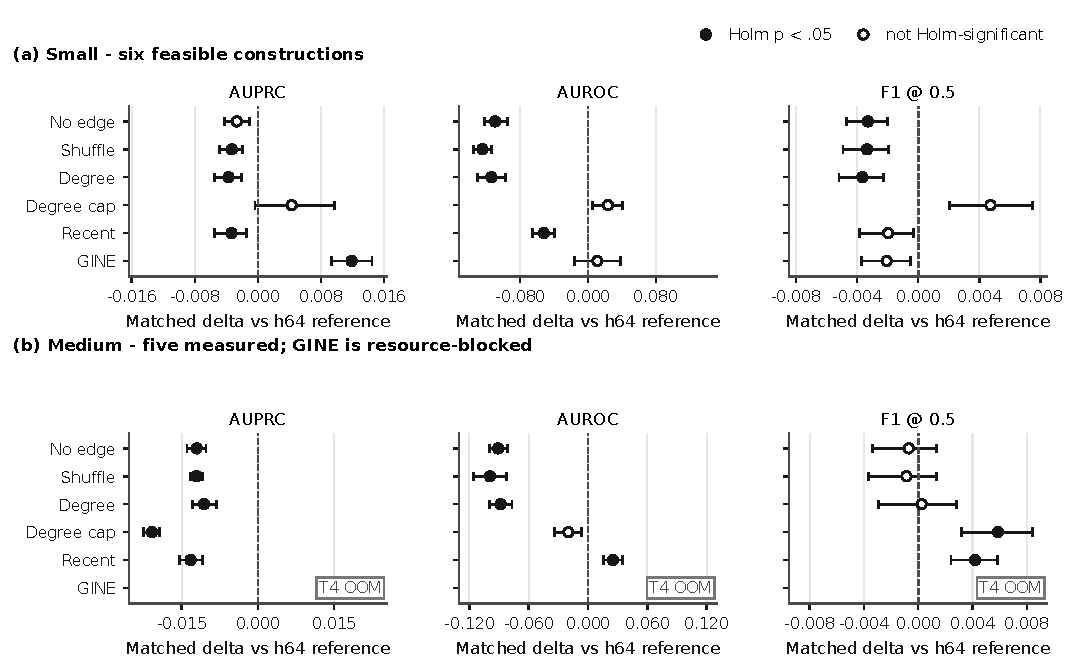
\includegraphics[width=0.88\textwidth]{fig05_matched_ablation_effects.pdf}
    \caption{Matched IBM effects relative to SAGE-edge h64. Intervals use ten seed blocks after fixed-context aggregation; Small-only GINE and blocked Medium cells are not pooled.}
    \label{fig:s-ibm-effects-v2}
\end{figure}

\subsection{Configuration-specific runtime and feasibility}

Table~\ref{tab:s-ibm-runtime-small} gives every Small configuration its own AUPRC and elapsed runner time.

\begingroup
\footnotesize
\setlength{\tabcolsep}{3pt}
\renewcommand{\arraystretch}{1.10}
\begin{longtable}{@{}p{0.11\textwidth} p{0.13\textwidth} p{0.19\textwidth} p{0.16\textwidth} r p{0.16\textwidth}@{}}
\caption{IBM Small configuration-level AUPRC, runtime, and feasibility.}\label{tab:s-ibm-runtime-small}\\
\toprule
\textbf{Variant} & \textbf{Protocol} & \textbf{Configuration} & \textbf{Status} & \textbf{AUPRC / seconds} & \textbf{Within-cell treatment} \\
\midrule
\endfirsthead
\caption[]{IBM Small configuration-level AUPRC, runtime, and feasibility. (continued)}\\
\toprule
\textbf{Variant} & \textbf{Protocol} & \textbf{Configuration} & \textbf{Status} & \textbf{AUPRC / seconds} & \textbf{Within-cell treatment} \\
\midrule
\endhead
\midrule
\multicolumn{6}{r}{\footnotesize Continued on next page}\\
\endfoot
\bottomrule
\endlastfoot
HI SMALL & Early-to-late & DegreeCap & \texttt{MEASURED\_\allowbreak{}FULL10} & 0.01285 / 27.89 & Pareto \\
HI SMALL & Early-to-late & DegreeOnly & \texttt{MEASURED\_\allowbreak{}FULL10} & 0.00513 / 31.61 & Measured, non-Pareto \\
HI SMALL & Early-to-late & GINE h64 & \texttt{MEASURED\_\allowbreak{}FULL10} & 0.02608 / 264.47 & Pareto \\
HI SMALL & Early-to-late & NoEdge & \texttt{MEASURED\_\allowbreak{}FULL10} & 0.00387 / 35.00 & Measured, non-Pareto \\
HI SMALL & Early-to-late & RecentWindow & \texttt{MEASURED\_\allowbreak{}FULL10} & 0.00496 / 16.64 & Pareto \\
HI SMALL & Early-to-late & SAGE-edge h64 & \texttt{MEASURED\_\allowbreak{}FULL10} & 0.01025 / 33.27 & Measured, non-Pareto \\
HI SMALL & Early-to-late & ShuffledEdge & \texttt{MEASURED\_\allowbreak{}FULL10} & 0.00412 / 32.52 & Measured, non-Pareto \\
HI SMALL & Late-window & DegreeCap & \texttt{MEASURED\_\allowbreak{}FULL10} & 0.02574 / 39.06 & Pareto \\
HI SMALL & Late-window & DegreeOnly & \texttt{MEASURED\_\allowbreak{}FULL10} & 0.00624 / 44.52 & Measured, non-Pareto \\
HI SMALL & Late-window & GINE h64 & \texttt{MEASURED\_\allowbreak{}FULL10} & 0.03125 / 363.32 & Pareto \\
HI SMALL & Late-window & NoEdge & \texttt{MEASURED\_\allowbreak{}FULL10} & 0.01052 / 48.70 & Measured, non-Pareto \\
HI SMALL & Late-window & RecentWindow & \texttt{MEASURED\_\allowbreak{}FULL10} & 0.00682 / 29.69 & Pareto \\
HI SMALL & Late-window & SAGE-edge h64 & \texttt{MEASURED\_\allowbreak{}FULL10} & 0.01100 / 47.21 & Measured, non-Pareto \\
HI SMALL & Late-window & ShuffledEdge & \texttt{MEASURED\_\allowbreak{}FULL10} & 0.00752 / 50.12 & Measured, non-Pareto \\
LI SMALL & Early-to-late & DegreeCap & \texttt{MEASURED\_\allowbreak{}FULL10} & 0.00389 / 42.79 & Pareto \\
LI SMALL & Early-to-late & DegreeOnly & \texttt{MEASURED\_\allowbreak{}FULL10} & 0.00168 / 48.76 & Measured, non-Pareto \\
LI SMALL & Early-to-late & GINE h64 & \texttt{MEASURED\_\allowbreak{}FULL10} & 0.00974 / 494.76 & Pareto \\
LI SMALL & Early-to-late & NoEdge & \texttt{MEASURED\_\allowbreak{}FULL10} & 0.00217 / 46.50 & Measured, non-Pareto \\
LI SMALL & Early-to-late & RecentWindow & \texttt{MEASURED\_\allowbreak{}FULL10} & 0.00225 / 27.39 & Pareto \\
LI SMALL & Early-to-late & SAGE-edge h64 & \texttt{MEASURED\_\allowbreak{}FULL10} & 0.00315 / 50.84 & Measured, non-Pareto \\
LI SMALL & Early-to-late & ShuffledEdge & \texttt{MEASURED\_\allowbreak{}FULL10} & 0.00199 / 46.62 & Measured, non-Pareto \\
LI SMALL & Late-window & DegreeCap & \texttt{MEASURED\_\allowbreak{}FULL10} & 0.00479 / 53.44 & Pareto \\
LI SMALL & Late-window & DegreeOnly & \texttt{MEASURED\_\allowbreak{}FULL10} & 0.00218 / 59.71 & Measured, non-Pareto \\
LI SMALL & Late-window & GINE h64 & \texttt{MEASURED\_\allowbreak{}FULL10} & 0.01060 / 675.32 & Pareto \\
LI SMALL & Late-window & NoEdge & \texttt{MEASURED\_\allowbreak{}FULL10} & 0.00283 / 58.44 & Measured, non-Pareto \\
LI SMALL & Late-window & RecentWindow & \texttt{MEASURED\_\allowbreak{}FULL10} & 0.00268 / 35.34 & Pareto \\
LI SMALL & Late-window & SAGE-edge h64 & \texttt{MEASURED\_\allowbreak{}FULL10} & 0.00568 / 65.92 & Pareto \\
LI SMALL & Late-window & ShuffledEdge & \texttt{MEASURED\_\allowbreak{}FULL10} & 0.00325 / 58.06 & Measured, non-Pareto \\
\end{longtable}
\noindent\footnotesize\emph{Scope and reading.} Pareto treatment is computed only within the same variant and protocol. Runtime is runner elapsed time, not a hardware-normalized complexity or energy measure. Blocked rows remain nonnumeric.\par
\endgroup


GINE takes approximately 9.1 times the h64 reference runtime in the aggregated Small comparison. Its higher AUPRC therefore does not imply universal deployability or dominance under every resource objective.

Table~\ref{tab:s-ibm-runtime-medium} gives the corresponding Medium cells and retains blocked GINE rows as nonnumeric statuses.

\begingroup
\footnotesize
\setlength{\tabcolsep}{3pt}
\renewcommand{\arraystretch}{1.10}
\begin{longtable}{@{}p{0.11\textwidth} p{0.13\textwidth} p{0.19\textwidth} p{0.16\textwidth} r p{0.16\textwidth}@{}}
\caption{IBM Medium configuration-level AUPRC, runtime, and feasibility.}\label{tab:s-ibm-runtime-medium}\\
\toprule
\textbf{Variant} & \textbf{Protocol} & \textbf{Configuration} & \textbf{Status} & \textbf{AUPRC / seconds} & \textbf{Within-cell treatment} \\
\midrule
\endfirsthead
\caption[]{IBM Medium configuration-level AUPRC, runtime, and feasibility. (continued)}\\
\toprule
\textbf{Variant} & \textbf{Protocol} & \textbf{Configuration} & \textbf{Status} & \textbf{AUPRC / seconds} & \textbf{Within-cell treatment} \\
\midrule
\endhead
\midrule
\multicolumn{6}{r}{\footnotesize Continued on next page}\\
\endfoot
\bottomrule
\endlastfoot
HI MEDIUM & Both Planned Protocols & GINE h64 & \texttt{RESOURCE\_\allowbreak{}BLOCKED\_\allowbreak{}T4\_\allowbreak{}CUDA\_\allowbreak{}OOM} & -- & Unmeasured \\
HI MEDIUM & Early-to-late & DegreeCap & \texttt{MEASURED\_\allowbreak{}FULL10} & 0.01186 / 216.79 & Measured, non-Pareto \\
HI MEDIUM & Early-to-late & DegreeOnly & \texttt{MEASURED\_\allowbreak{}FULL10} & 0.02524 / 238.96 & Pareto \\
HI MEDIUM & Early-to-late & NoEdge & \texttt{MEASURED\_\allowbreak{}FULL10} & 0.02447 / 248.13 & Measured, non-Pareto \\
HI MEDIUM & Early-to-late & RecentWindow & \texttt{MEASURED\_\allowbreak{}FULL10} & 0.01866 / 128.15 & Pareto \\
HI MEDIUM & Early-to-late & SAGE-edge h64 & \texttt{MEASURED\_\allowbreak{}FULL10} & 0.04242 / 249.73 & Pareto \\
HI MEDIUM & Early-to-late & ShuffledEdge & \texttt{MEASURED\_\allowbreak{}FULL10} & 0.02388 / 255.57 & Measured, non-Pareto \\
HI MEDIUM & Late-window & DegreeCap & \texttt{MEASURED\_\allowbreak{}FULL10} & 0.01274 / 261.86 & Measured, non-Pareto \\
HI MEDIUM & Late-window & DegreeOnly & \texttt{MEASURED\_\allowbreak{}FULL10} & 0.03262 / 290.36 & Pareto \\
HI MEDIUM & Late-window & NoEdge & \texttt{MEASURED\_\allowbreak{}FULL10} & 0.02989 / 298.87 & Measured, non-Pareto \\
HI MEDIUM & Late-window & RecentWindow & \texttt{MEASURED\_\allowbreak{}FULL10} & 0.02895 / 153.10 & Pareto \\
HI MEDIUM & Late-window & SAGE-edge h64 & \texttt{MEASURED\_\allowbreak{}FULL10} & 0.04998 / 301.12 & Pareto \\
HI MEDIUM & Late-window & ShuffledEdge & \texttt{MEASURED\_\allowbreak{}FULL10} & 0.02970 / 311.00 & Measured, non-Pareto \\
LI MEDIUM & Both Planned Protocols & GINE h64 & \texttt{RESOURCE\_\allowbreak{}BLOCKED\_\allowbreak{}T4\_\allowbreak{}CUDA\_\allowbreak{}OOM} & -- & Unmeasured \\
LI MEDIUM & Early-to-late & DegreeCap & \texttt{MEASURED\_\allowbreak{}FULL10} & 0.00316 / 211.08 & Measured, non-Pareto \\
LI MEDIUM & Early-to-late & DegreeOnly & \texttt{MEASURED\_\allowbreak{}FULL10} & 0.00568 / 253.30 & Measured, non-Pareto \\
LI MEDIUM & Early-to-late & NoEdge & \texttt{MEASURED\_\allowbreak{}FULL10} & 0.00515 / 243.66 & Measured, non-Pareto \\
LI MEDIUM & Early-to-late & RecentWindow & \texttt{MEASURED\_\allowbreak{}FULL10} & 0.00657 / 129.07 & Pareto \\
LI MEDIUM & Early-to-late & SAGE-edge h64 & \texttt{MEASURED\_\allowbreak{}FULL10} & 0.01030 / 249.24 & Pareto \\
LI MEDIUM & Early-to-late & ShuffledEdge & \texttt{MEASURED\_\allowbreak{}FULL10} & 0.00551 / 246.03 & Measured, non-Pareto \\
LI MEDIUM & Late-window & DegreeCap & \texttt{MEASURED\_\allowbreak{}FULL10} & 0.00256 / 251.89 & Measured, non-Pareto \\
LI MEDIUM & Late-window & DegreeOnly & \texttt{MEASURED\_\allowbreak{}FULL10} & 0.00778 / 303.13 & Measured, non-Pareto \\
LI MEDIUM & Late-window & NoEdge & \texttt{MEASURED\_\allowbreak{}FULL10} & 0.00600 / 294.95 & Measured, non-Pareto \\
LI MEDIUM & Late-window & RecentWindow & \texttt{MEASURED\_\allowbreak{}FULL10} & 0.00661 / 156.28 & Pareto \\
LI MEDIUM & Late-window & SAGE-edge h64 & \texttt{MEASURED\_\allowbreak{}FULL10} & 0.01105 / 300.67 & Pareto \\
LI MEDIUM & Late-window & ShuffledEdge & \texttt{MEASURED\_\allowbreak{}FULL10} & 0.00634 / 294.61 & Measured, non-Pareto \\
\end{longtable}
\noindent\footnotesize\emph{Scope and reading.} Pareto treatment is computed only within the same variant and protocol. Runtime is runner elapsed time, not a hardware-normalized complexity or energy measure. Blocked rows remain nonnumeric.\par
\endgroup


RecentWindow reduces aggregated Medium mean runtime from 275.19 to 141.65 seconds, while changing AUPRC by \(-0.01324\), AUROC by \(+0.02525\), and F1 by \(+0.00419\). Pareto flags are computed only within the same variant/protocol cell. Runtime is not normalized across hardware or implementations.

\paragraph{Sensitivity location.}
The complete context rows, including reference/candidate means, intervals, effect sizes, descriptive p-values, and source paths, remain at \path{results/tkde_rebuild/IBM_MATCHED_ABLATION_CONTEXT_EFFECTS.csv}. Their checksum and schema are reported in Table~\ref{tab:s-raw-artifacts}.

\section{Rank-versus-decision analyses}
\label{sec:s-rank-decision}

\subsection{Baseline-grid disagreement}

Table~\ref{tab:s-rank-baseline_grid} compares AUPRC and fixed-threshold F1 winners in the eight baseline contexts. The feasible set contains the same three configurations in every row.

\begin{table}[tbp]
\centering
\footnotesize
\setlength{\tabcolsep}{3.2pt}
\renewcommand{\arraystretch}{1.12}
\caption{IBM baseline grid: AUPRC and F1@0.5 winners and rank agreement.}
\label{tab:s-rank-baseline_grid}
\begin{tabularx}{\textwidth}{@{}>{\raggedright\arraybackslash}p{0.11\textwidth} >{\raggedright\arraybackslash}p{0.13\textwidth} r Y Y r l@{}}
\toprule
\textbf{Variant} & \textbf{Protocol} & \textbf{Feasible n} & \textbf{AUPRC winner} & \textbf{F1 winner} & \textbf{$\rho$} & \textbf{Disagree} \\
\midrule
HI MEDIUM & Early-to-late & 3 & HistGB & HistGB & 1.000 & No \\
HI MEDIUM & Late-window & 3 & HistGB & LogReg & -1.000 & Yes \\
HI SMALL & Early-to-late & 3 & HistGB & HistGB & 1.000 & No \\
HI SMALL & Late-window & 3 & HistGB & HistGB & 1.000 & No \\
LI MEDIUM & Early-to-late & 3 & HistGB & SAGE-edge h32 & -0.500 & Yes \\
LI MEDIUM & Late-window & 3 & HistGB & SAGE-edge h32 & -0.500 & Yes \\
LI SMALL & Early-to-late & 3 & HistGB & HistGB & 1.000 & No \\
LI SMALL & Late-window & 3 & HistGB & HistGB & 1.000 & No \\
\bottomrule
\end{tabularx}
\vspace{2pt}
\begin{minipage}{\textwidth}\footnotesize\emph{Scope and reading.} Spearman correlation is computed over the exact feasible set in each row. F1 uses the saved threshold of 0.5; disagreement is not asserted to be threshold-invariant.\end{minipage}
\end{table}


The AUPRC and F1 winners differ in 3 of 8 baseline contexts. This is not a contradiction: AUPRC summarizes the score ordering, while F1 evaluates one threshold. Rank correlation is shown to expose the magnitude of agreement rather than only a categorical winner change.

\subsection{Graph-grid disagreement}

Table~\ref{tab:s-rank-graph_grid} performs the same comparison in the exact feasible graph-construction set.

\begin{table}[tbp]
\centering
\footnotesize
\setlength{\tabcolsep}{3.2pt}
\renewcommand{\arraystretch}{1.12}
\caption{IBM graph grid: AUPRC and F1@0.5 winners and rank agreement.}
\label{tab:s-rank-graph_grid}
\begin{tabularx}{\textwidth}{@{}>{\raggedright\arraybackslash}p{0.11\textwidth} >{\raggedright\arraybackslash}p{0.13\textwidth} r Y Y r l@{}}
\toprule
\textbf{Variant} & \textbf{Protocol} & \textbf{Feasible n} & \textbf{AUPRC winner} & \textbf{F1 winner} & \textbf{$\rho$} & \textbf{Disagree} \\
\midrule
HI MEDIUM & Early-to-late & 6 & SAGE-edge h64 & DegreeCap & -0.486 & Yes \\
HI MEDIUM & Late-window & 6 & SAGE-edge h64 & DegreeCap & -0.771 & Yes \\
HI SMALL & Early-to-late & 7 & GINE h64 & DegreeCap & 0.857 & Yes \\
HI SMALL & Late-window & 7 & GINE h64 & DegreeCap & 0.786 & Yes \\
LI MEDIUM & Early-to-late & 6 & SAGE-edge h64 & DegreeCap & -0.086 & Yes \\
LI MEDIUM & Late-window & 6 & SAGE-edge h64 & DegreeCap & -0.029 & Yes \\
LI SMALL & Early-to-late & 7 & GINE h64 & DegreeCap & 0.607 & Yes \\
LI SMALL & Late-window & 7 & GINE h64 & DegreeCap & 0.571 & Yes \\
\bottomrule
\end{tabularx}
\vspace{2pt}
\begin{minipage}{\textwidth}\footnotesize\emph{Scope and reading.} Spearman correlation is computed over the exact feasible set in each row. F1 uses the saved threshold of 0.5; disagreement is not asserted to be threshold-invariant.\end{minipage}
\end{table}


The winners differ in all 8 graph-grid contexts, giving 11 of 16 disagreements across the two families. For example, in HI-Medium late-window, SAGE-edge h64 ranks first by AUPRC but sixth by F1; DegreeCap ranks sixth by AUPRC but first by F1. Medium GINE is not in the feasible set, and the sender-receiver identity row is not counted as an independent method.

\begin{figure}[tbp]
    \centering
    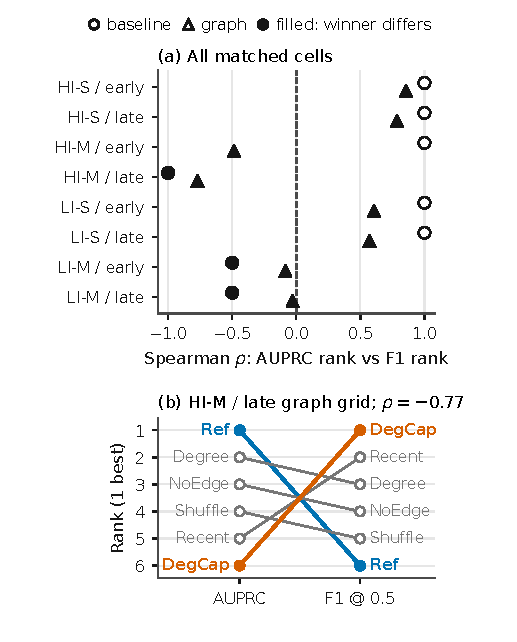
\includegraphics[width=0.84\textwidth]{fig04_rank_decision_divergence.pdf}
    \caption{AUPRC and F1@0.5 rank divergence within exact IBM feasibility sets. The plot makes the operating-point dependence visible without pooling scales or blocked configurations.}
    \label{fig:s-rank-divergence-v2}
\end{figure}

\paragraph{Interpretive limit.}
The count 11 of 16 is specific to threshold 0.5. It does not establish disagreement under every threshold or review budget, and higher AUROC does not automatically imply better operational decisions.

\section{Review-budget and calibration diagnostics}
\label{sec:s-review-calibration}

\subsection{One-percent review capacity}

Review-budget metrics ask how much fraud is found when only the top \(b\%\) of scores can be reviewed. Table~\ref{tab:s-review-budget-1pct} reports the central 1\% operating point for five saved-prediction policies on each dataset.

\begin{table}[tbp]
\centering
\footnotesize
\setlength{\tabcolsep}{3.2pt}
\renewcommand{\arraystretch}{1.12}
\caption{Precision and recall at a 1\% review budget.}
\label{tab:s-review-budget-1pct}
\begin{tabularx}{\textwidth}{@{}>{\raggedright\arraybackslash}p{0.14\textwidth} Y r r r r@{}}
\toprule
\textbf{Dataset} & \textbf{Policy} & \textbf{n} & \textbf{Precision} & \textbf{SD} & \textbf{Recall (SD)} \\
\midrule
DGraphFin & Best validation branch & 10 & 0.0150 & 0.0058 & 0.0138 (0.0053) \\
DGraphFin & Feature branch & 10 & 0.0161 & 0.0124 & 0.0147 (0.0114) \\
DGraphFin & Graph branch & 10 & 0.0150 & 0.0058 & 0.0138 (0.0053) \\
DGraphFin & GraphSafe conservative & 10 & 0.0229 & 0.0062 & 0.0209 (0.0056) \\
DGraphFin & Simple average & 10 & 0.0156 & 0.0078 & 0.0143 (0.0071) \\
Elliptic & Best validation branch & 10 & 0.7785 & 0.0482 & 0.1201 (0.0074) \\
Elliptic & Feature branch & 10 & 0.6481 & 0.0635 & 0.0999 (0.0098) \\
Elliptic & Graph branch & 10 & 0.8353 & 0.0359 & 0.1288 (0.0055) \\
Elliptic & GraphSafe conservative & 10 & 0.7624 & 0.0432 & 0.1176 (0.0067) \\
Elliptic & Simple average & 10 & 0.8276 & 0.0556 & 0.1276 (0.0086) \\
\bottomrule
\end{tabularx}
\vspace{2pt}
\begin{minipage}{\textwidth}\footnotesize\emph{Scope and reading.} The six model/protocol contexts are averaged within seed before the ten-seed summary. Review-budget results are capacity-conditioned and do not replace AUPRC.\end{minipage}
\end{table}


On DGraphFin, GraphSafe conservative averages precision 0.0229 and recall 0.0209, compared with 0.0156 and 0.0143 for simple averaging. On Elliptic, the direction reverses: GraphSafe averages precision 0.7624 and recall 0.1176, while simple averaging reaches 0.8274 and 0.1276. The complete 0.5\%, 1\%, and 2\% rows remain in \path{results/tkde_rebuild/REVIEW_BUDGET_CURVES.csv}.

\begin{figure}[tbp]
    \centering
    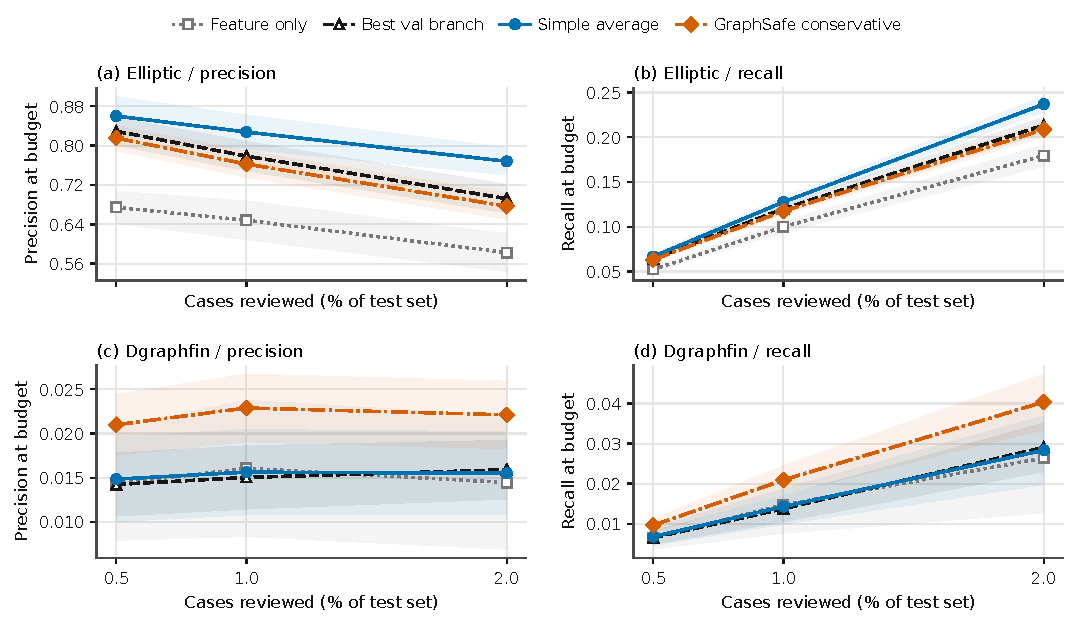
\includegraphics[width=0.88\textwidth]{fig07_review_budget_analysis.pdf}
    \caption{Precision and recall across the three declared review capacities. Uncertainty uses ten seed blocks after averaging six fixed contexts within seed.}
    \label{fig:s-review-budget-v2}
\end{figure}

\subsection{Calibration}

Table~\ref{tab:s-calibration} reports ECE and Brier score from saved predictions.

\begin{table}[tbp]
\centering
\footnotesize
\setlength{\tabcolsep}{3.2pt}
\renewcommand{\arraystretch}{1.12}
\caption{Saved-prediction calibration diagnostics.}
\label{tab:s-calibration}
\begin{tabularx}{\textwidth}{@{}>{\raggedright\arraybackslash}p{0.14\textwidth} Y r r r r@{}}
\toprule
\textbf{Dataset} & \textbf{Policy} & \textbf{n} & \textbf{ECE} & \textbf{SD} & \textbf{Brier (SD)} \\
\midrule
DGraphFin & Best validation branch & 10 & 0.28443 & 0.02093 & 0.09632 (0.01160) \\
DGraphFin & Feature branch & 10 & 0.28076 & 0.02877 & 0.09356 (0.01546) \\
DGraphFin & Graph branch & 10 & 0.28443 & 0.02093 & 0.09632 (0.01160) \\
DGraphFin & GraphSafe conservative & 10 & 0.27507 & 0.02032 & 0.09094 (0.01054) \\
DGraphFin & Simple average & 10 & 0.28260 & 0.02234 & 0.09295 (0.01241) \\
Elliptic & Best validation branch & 10 & 0.08760 & 0.01392 & 0.07341 (0.00807) \\
Elliptic & Feature branch & 10 & 0.13074 & 0.00643 & 0.09912 (0.00441) \\
Elliptic & Graph branch & 10 & 0.07298 & 0.00779 & 0.06515 (0.00580) \\
Elliptic & GraphSafe conservative & 10 & 0.09820 & 0.01727 & 0.07899 (0.00848) \\
Elliptic & Simple average & 10 & 0.09631 & 0.00381 & 0.07059 (0.00255) \\
\bottomrule
\end{tabularx}
\vspace{2pt}
\begin{minipage}{\textwidth}\footnotesize\emph{Scope and reading.} ECE uses ten bins and is descriptive. These fixed-dataset summaries do not establish calibrated probabilities in a deployment population.\end{minipage}
\end{table}


On DGraphFin, GraphSafe's mean ECE is 0.2751 and Brier score is 0.09094, compared with 0.2826 and 0.09295 for simple averaging. On Elliptic, simple averaging is better on both diagnostics (ECE 0.09631 versus 0.09820; Brier 0.07059 versus 0.07899).

\paragraph{Limit.}
These are fixed-dataset diagnostics, not guarantees of calibration in a bank population. Capacity, delayed labels, investigator actions, and changing prevalence can alter the operating surface.

\section{GraphSafe-TTA case study}
\label{sec:s-graphsafe-v2}

\subsection{Policy definition}

GraphSafe is a post-training switch over aligned feature and graph prediction files. It does not retrain either branch. For each prediction it combines absolute score disagreement, within-split percentile-rank disagreement, and mean binary entropy. Validation-set 95th percentiles scale the terms:
\begin{equation}
 \rho_i=\frac{d_i^{\mathrm{score}}/a_s+d_i^{\mathrm{rank}}/a_r+
 0.5h_i/a_h}{2.5}.
\end{equation}
A validation search chooses cutoff \(\gamma\) and decision threshold \(\tau\), and
\begin{equation}
 q_i^{\mathrm{GS}}=
 \begin{cases}
 q_i^{\mathrm{graph}}, & \rho_i\leq\gamma,\\
 q_i^{\mathrm{feature}}, & \rho_i>\gamma.
 \end{cases}
\end{equation}
Test labels are used only for final evaluation. Comparators include each branch, the validation-selected branch, and simple averaging. Additional saved-output diagnostics use validation-weighted averaging, temperature scaling, prior correction, and rolling thresholds~\cite{guo2017calibration,saerens2002prior,geifman2017selective}.

\subsection{Aggregate policy outcomes}

Table~\ref{tab:s-graphsafe-summary} first averages six graph-model/protocol contexts within seed and then summarizes ten seeds.

\begingroup
\footnotesize
\setlength{\tabcolsep}{3pt}
\renewcommand{\arraystretch}{1.10}
\begin{longtable}{@{}p{0.12\textwidth} p{0.19\textwidth} r r r r r@{}}
\caption{GraphSafe and comparator outcomes after seed-block aggregation.}\label{tab:s-graphsafe-summary}\\
\toprule
\textbf{Dataset} & \textbf{Policy} & \textbf{n} & \textbf{F1} & \textbf{AUPRC} & \textbf{Recall@1\%} & \textbf{Cost risk} \\
\midrule
\endfirsthead
\caption[]{GraphSafe and comparator outcomes after seed-block aggregation. (continued)}\\
\toprule
\textbf{Dataset} & \textbf{Policy} & \textbf{n} & \textbf{F1} & \textbf{AUPRC} & \textbf{Recall@1\%} & \textbf{Cost risk} \\
\midrule
\endhead
\midrule
\multicolumn{7}{r}{\footnotesize Continued on next page}\\
\endfoot
\bottomrule
\endlastfoot
DGraphFin & Best validation branch & 10 & 0.03624 & 0.01641 & 0.01375 & 0.47266 \\
DGraphFin & Feature branch & 10 & 0.03241 & 0.01390 & 0.01469 & 0.59243 \\
DGraphFin & Graph branch & 10 & 0.03624 & 0.01641 & 0.01375 & 0.47266 \\
DGraphFin & GraphSafe conservative & 10 & 0.04257 & 0.01901 & 0.02092 & 0.29128 \\
DGraphFin & Simple average & 10 & 0.03647 & 0.01625 & 0.01430 & 0.45220 \\
Elliptic & Best validation branch & 10 & 0.53247 & 0.49281 & 0.12005 & 0.17972 \\
Elliptic & Feature branch & 10 & 0.51700 & 0.43718 & 0.09994 & 0.17929 \\
Elliptic & Graph branch & 10 & 0.53252 & 0.51525 & 0.12881 & 0.18203 \\
Elliptic & GraphSafe conservative & 10 & 0.53325 & 0.48762 & 0.11756 & 0.17831 \\
Elliptic & Simple average & 10 & 0.55130 & 0.53292 & 0.12762 & 0.17086 \\
\end{longtable}
\noindent\footnotesize\emph{Scope and reading.} Each row averages six fixed contexts within seed, then summarizes ten seeds. The 1:5 cost is illustrative. DGraphFin descriptive gains and Elliptic negative comparisons are both retained.\par
\endgroup


On DGraphFin, GraphSafe conservative has mean F1 0.04257, AUPRC 0.01901, Recall@1\% 0.02092, and cost risk 0.29128; simple averaging has 0.03647, 0.01625, 0.01430, and 0.45220. On Elliptic, simple averaging is stronger on F1 (0.55130 versus 0.53325), AUPRC (0.53292 versus 0.48762), Recall@1\% (0.12762 versus 0.11756), and cost risk (0.17086 versus 0.17831). Both the favorable and negative comparisons are central to the bounded interpretation.

\subsection{Multiplicity-aware comparison}

Table~\ref{tab:s-graphsafe-paired} reports the 12 GraphSafe-conservative contrasts against simple averaging. The full correction family contains 48 comparator-metric tests.

\begingroup
\footnotesize
\setlength{\tabcolsep}{3pt}
\renewcommand{\arraystretch}{1.10}
\begin{longtable}{@{}p{0.13\textwidth} p{0.20\textwidth} p{0.09\textwidth} r p{0.25\textwidth} r@{}}
\caption{GraphSafe conservative minus simple-average paired effects.}\label{tab:s-graphsafe-paired}\\
\toprule
\textbf{Dataset} & \textbf{Metric} & \textbf{Direction} & \textbf{$\Delta$} & \textbf{95\% CI} & \textbf{Holm p} \\
\midrule
\endfirsthead
\caption[]{GraphSafe conservative minus simple-average paired effects. (continued)}\\
\toprule
\textbf{Dataset} & \textbf{Metric} & \textbf{Direction} & \textbf{$\Delta$} & \textbf{95\% CI} & \textbf{Holm p} \\
\midrule
\endhead
\midrule
\multicolumn{6}{r}{\footnotesize Continued on next page}\\
\endfoot
\bottomrule
\endlastfoot
DGraphFin & auprc & higher & +0.00275 & [0.00113, 0.00451] & 0.3906 \\
DGraphFin & average block regret & lower & +0.16112 & [0.06278, 0.28531] & 0.2246 \\
DGraphFin & cost sensitive risk & lower & +0.16092 & [0.06409, 0.28513] & 0.2246 \\
DGraphFin & f1 & higher & +0.00610 & [0.00370, 0.00868] & 0.1094 \\
DGraphFin & recall at 1pct & higher & +0.00662 & [0.00402, 0.00944] & 0.0938 \\
DGraphFin & worst block regret & lower & +0.16603 & [0.06420, 0.29419] & 0.2246 \\
Elliptic & auprc & higher & -0.04530 & [-0.05466, -0.03622] & 0.0938 \\
Elliptic & average block regret & lower & -0.00667 & [-0.00825, -0.00515] & 0.0938 \\
Elliptic & cost sensitive risk & lower & -0.00745 & [-0.00887, -0.00610] & 0.0938 \\
Elliptic & f1 & higher & -0.01804 & [-0.02384, -0.01223] & 0.0938 \\
Elliptic & recall at 1pct & higher & -0.01006 & [-0.01371, -0.00648] & 0.1094 \\
Elliptic & worst block regret & lower & -0.03058 & [-0.04066, -0.01922] & 0.1094 \\
\end{longtable}
\noindent\footnotesize\emph{Scope and reading.} The correction family contains all 48 saved-prediction comparator tests, not only the 12 rows shown here. No adjusted p-value is below 0.05; therefore this case does not establish universal dominance or ranking repair.\par
\endgroup


The DGraphFin GraphSafe AUPRC difference is 0.00275 with 95\% CI \([0.00113,0.00451]\), but Holm \(p=0.3906\). The Elliptic difference is \(-0.04530\), CI \([-0.05466,-0.03622]\), with Holm \(p=0.0938\). No one of the 48 adjusted tests is below 0.05.

\paragraph{What this case establishes.}
The saved-output surface demonstrates how a typed support system retains mixed operational evidence and strong comparators. It does not establish universal GraphSafe dominance, ranking repair, automatic AML deployment, or a correction of rank metrics by calibration.

\section{Resource-boundary case studies}
\label{sec:s-resource-cases-v2}

The resource coordinate records what was attempted under which envelope and how the benchmark treats the outcome. Table~\ref{tab:s-resource-cases} is the compact index; the five cases below give the reviewer-facing interpretation.

\begingroup
\footnotesize
\setlength{\tabcolsep}{3pt}
\renewcommand{\arraystretch}{1.10}
\begin{longtable}{@{}p{0.21\textwidth} p{0.21\textwidth} p{0.11\textwidth} p{0.15\textwidth} p{0.18\textwidth}@{}}
\caption{Measured resource outcomes and benchmark treatment.}\label{tab:s-resource-cases}\\
\toprule
\textbf{Evaluation cell} & \textbf{Declared envelope / observed event} & \textbf{Outputs} & \textbf{Status} & \textbf{Benchmark treatment} \\
\midrule
\endfirsthead
\caption[]{Measured resource outcomes and benchmark treatment. (continued)}\\
\toprule
\textbf{Evaluation cell} & \textbf{Declared envelope / observed event} & \textbf{Outputs} & \textbf{Status} & \textbf{Benchmark treatment} \\
\midrule
\endhead
\midrule
\multicolumn{5}{r}{\footnotesize Continued on next page}\\
\endfoot
\bottomrule
\endlastfoot
IBM AML HI-Large & safe resource guard & 0 results; 0 predictions & \texttt{SAFE\_\allowbreak{}RESOURCE\_\allowbreak{}BLOCKED} & not in predictive ranking \\
IBM AML LI-Large & safe resource guard & 0 results; 0 predictions & \texttt{SAFE\_\allowbreak{}RESOURCE\_\allowbreak{}BLOCKED} & not in predictive ranking \\
IBM AML HI-Medium GINE h64 & single Tesla T4 CUDA OOM & 0 of 20 planned results; 0 predictions & \texttt{RESOURCE\_\allowbreak{}BLOCKED\_\allowbreak{}T4\_\allowbreak{}CUDA\_\allowbreak{}OOM} & not in predictive ranking \\
IBM AML LI-Medium GINE h64 & single Tesla T4 CUDA OOM & 0 of 20 planned results; 0 predictions & \texttt{RESOURCE\_\allowbreak{}BLOCKED\_\allowbreak{}T4\_\allowbreak{}CUDA\_\allowbreak{}OOM} & not in predictive ranking \\
DGraphFin GAT h64/l2 & Tesla T4 CUDA OOM & 0 of 20 planned results; 0 predictions & \texttt{BLOCKED\_\allowbreak{}T4\_\allowbreak{}OOM} & memory-reduced h32/l1 diagnostic is not a replacement \\
DGraphFin GraphSAGE max-pool rerun & larger GPU required & 0 results; 0 predictions & \texttt{BLOCKED\_\allowbreak{}WAITING\_\allowbreak{}FOR\_\allowbreak{}GPU} & no imported result CSV \\
\end{longtable}
\noindent\footnotesize\emph{Scope and reading.} A blocked cell is unmeasured and excluded from predictive ranks, matched means, and Pareto sets. A reduced diagnostic cannot replace a fixed blocked configuration.\par
\endgroup


\subsection{IBM AML Large guards}

HI-Large and LI-Large stopped at the safe resource guard and produced zero result and prediction files. Evidence exists for the guard and planned configuration; predictive evidence does not exist. The safe wording is that Large lies outside the admitted resource envelope and is unmeasured. It is not permissible to rank Large, infer underperformance, or claim full-10 coverage.

\subsection{Medium GINE T4 out-of-memory}

HI-Medium and LI-Medium GINE h64 each encountered single-T4 CUDA OOM and produced zero of 20 planned outputs. Small GINE performance and the Medium failure record both exist. Medium GINE performance does not. It is excluded from Medium winner sets, matched means, and Pareto sets rather than imputed.

\subsection{Fixed DGraphFin GAT T4 out-of-memory}

The fixed h64/l2 GAT lane has zero of 20 planned results and predictions under the T4 envelope. A memory-reduced h32/l1 diagnostic changes architecture and cannot substitute for the blocked fixed cell. The benchmark may compare their feasibility statuses, not their predictive scores.

\subsection{RB18 and larger-GPU extension status}

The DGraphFin GraphSAGE max-pool extension has preparation commands and status files but no imported result CSV. A larger GPU was requested; no validated runtime record establishes P100, A100, or H100 performance. The safe wording is waiting-for-GPU/unmeasured, not hardware-backed evidence.

\subsection{Memory-reduced exploratory architectures}

Memory-reduced variants can diagnose whether a code path runs under a smaller envelope. They remain exploratory because width, depth, sampling, or features differ from the fixed target. Directory presence, notebook generation, or partial predictions cannot fill a claim scoped to the original architecture.

\subsection{False-promotion protections}

Table~\ref{tab:s-false-promotions-v2} explains how count-only logic could incorrectly promote failed imports, duplicate labels, aliases, diagnostics, and zero-output plans.

\begingroup
\footnotesize
\setlength{\tabcolsep}{3pt}
\renewcommand{\arraystretch}{1.10}
\begin{longtable}{@{}p{0.08\textwidth} p{0.22\textwidth} r r p{0.20\textwidth} p{0.19\textwidth}@{}}
\caption{False-promotion patterns guarded by the artifact layer.}\label{tab:s-false-promotions-v2}\\
\toprule
\textbf{Audit} & \textbf{Family} & \textbf{Result risk} & \textbf{Prediction risk} & \textbf{Correct treatment} & \textbf{Why count-only logic fails} \\
\midrule
\endfirsthead
\caption[]{False-promotion patterns guarded by the artifact layer. (continued)}\\
\toprule
\textbf{Audit} & \textbf{Family} & \textbf{Result risk} & \textbf{Prediction risk} & \textbf{Correct treatment} & \textbf{Why count-only logic fails} \\
\midrule
\endhead
\midrule
\multicolumn{6}{r}{\footnotesize Continued on next page}\\
\endfoot
\bottomrule
\endlastfoot
FP01 & V22 failed/noncomparable imports & 38 & 38 & \texttt{EXCLUDED\_\allowbreak{}INTEGRITY} & missing seed, failed return-code, duplicate/conflicting merge metadata \\
FP02 & V24 RB41 duplicate stress labels & 240 & 240 & \texttt{DEDUPLICATE\_\allowbreak{}TO\_\allowbreak{}120\_\allowbreak{}BASE\_\allowbreak{}CELLS} & stress label is never passed to benchmark harness; all performance metrics repeat \\
FP03 & V24 memory-reduced DGraphFin GAT h32/l1 & 20 & 20 & \texttt{DIAGNOSTIC\_\allowbreak{}ONLY} & different width/depth; canonical lock says not comparable \\
FP04 & V26 legacy P100-named lane & 12 & 12 & \texttt{NORMALIZE\_\allowbreak{}ALIAS\_\allowbreak{}TO\_\allowbreak{}T4/\allowbreak{}CUDA0} & runtime records identify cuda:0 and validation normalizes the alias; path names are not hardware evidence \\
FP05 & IBM AML Large status/runbook artifacts & 0 & 0 & \texttt{RESOURCE\_\allowbreak{}BLOCKED} & canonical lock contains zero results and predictions \\
FP06 & Medium GINE blocked plans & 0 & 0 & \texttt{RESOURCE\_\allowbreak{}BLOCKED} & two T4-OOM rows; zero results and predictions \\
FP07 & RB18 larger-GPU preparation & 0 & 0 & \texttt{BLOCKED\_\allowbreak{}WAITING\_\allowbreak{}FOR\_\allowbreak{}GPU} & validation reports no imported result CSV \\
\end{longtable}
\noindent\footnotesize\emph{Scope and reading.} The 310 result and 310 prediction files at risk are not additional evidence. Zero-output plans remain visible because directories and notebooks can otherwise be mistaken for completed runs.\par
\endgroup


Across metric-bearing artifacts, 310 result and 310 prediction files are at risk of naive promotion. The count includes 240 duplicate V24 labels, 38 failed/noncomparable V22 imports, 20 memory-reduced GAT diagnostics, and 12 legacy hardware-alias files. These remain provenance or validation cases, not additional performance evidence.

\paragraph{General treatment.}
Resource-blocked cells are unmeasured and predictively unordered. A future run on different hardware could produce evidence, but no direction follows from that possibility.

\section{Claim ledger and provenance map}
\label{sec:s-claims-v2}

The frozen ledger contains 22 typed claims: 12 supported, three diagnostic-only, two refuted-in-scope, two resource-blocked, two supported theoretically, and one supported with a resource boundary. The following five tables preserve every claim ID, exact scope string, status, permitted wording, and prohibited generalization exactly once. Full matched evidence-unit identifiers remain in the machine-readable ledger.

\subsection{Protocol and architecture claims}

\begin{table}[tbp]
\centering
\footnotesize
\setlength{\tabcolsep}{3.2pt}
\renewcommand{\arraystretch}{1.12}
\caption{Protocol and architecture claims.}
\label{tab:s-claims-protocol}
\begin{tabularx}{\textwidth}{@{}l >{\raggedright\arraybackslash}p{0.16\textwidth} Y Y Y@{}}
\toprule
\textbf{ID} & \textbf{Status} & \textbf{Exact scoped subject} & \textbf{Permitted wording} & \textbf{Prohibited generalization} \\
\midrule
C01 & \texttt{SUPPORTED} & Elliptic; MLP/GCN/GraphSAGE; strict versus isolated; seeds 1-10 & the evaluated Elliptic leaderboard reverses at the top under the two visibility contracts & evaluation protocols always reverse rankings \\
C02 & \texttt{SUPPORTED} & Elliptic and DGraphFin; MLP; strict versus isolated; seeds 1-10 & the MLP negative control is unchanged by the graph-only visibility intervention & the two protocols are identical \\
C03 & \texttt{SUPPORTED} & Elliptic and DGraphFin; GCN and GraphSAGE; strict versus isolated; seeds 1-10 & effects depend on architecture and dataset in the evaluated grid & graph isolation is always harmful or always beneficial \\
C04 & \texttt{REFUTED\_\allowbreak{}IN\_\allowbreak{}SCOPE} & all datasets, constructions, protocols, and graph models & the evaluated evidence rejects a uniform graph-harm narrative & GNNs fail universally; graph methods are always harmful \\
C19 & \texttt{SUPPORTED\_\allowbreak{}THEORETICALLY} & typed deployment contracts & protocol results are contract-relative & any numerical difference is caused solely by graph visibility \\
\bottomrule
\end{tabularx}
\vspace{2pt}
\begin{minipage}{\textwidth}\footnotesize\emph{Scope and reading.} Status and scope text are copied from the frozen 22-claim ledger. Exact matched evidence-unit identifiers remain in the machine-readable ledger rather than in these reviewer-facing cells.\end{minipage}
\end{table}


These claims distinguish an observed Elliptic top-rank reversal and architecture-dependent visibility effects from the prohibited universal graph-harm narrative. C19 further prevents results from contracts with different claim-relevant coordinates from being treated as interchangeable.

\subsection{IBM baseline, construction, and scale claims}

\begin{table}[tbp]
\centering
\footnotesize
\setlength{\tabcolsep}{3.2pt}
\renewcommand{\arraystretch}{1.12}
\caption{IBM AML baseline, construction, and scale claims.}
\label{tab:s-claims-ibm}
\begin{tabularx}{\textwidth}{@{}l >{\raggedright\arraybackslash}p{0.16\textwidth} Y Y Y@{}}
\toprule
\textbf{ID} & \textbf{Status} & \textbf{Exact scoped subject} & \textbf{Permitted wording} & \textbf{Prohibited generalization} \\
\midrule
C05 & \texttt{SUPPORTED} & IBM AML HI/LI Small/Medium; two temporal protocols; HistGB/LogReg/GraphSAGE-h32; seeds 1-10 & HistGB leads mean AUPRC in all eight evaluated baseline-grid contexts & trees are universally best for AML \\
C07 & \texttt{SUPPORTED} & HI/LI Small/Medium; both protocols; edge-aware GraphSAGE h64 versus NoEdge/ShuffledEdge; seeds 1-10 & the original edge-feature representation outperforms the two matched controls on mean AUPRC in this grid & edge features causally improve all fraud models \\
C08 & \texttt{SUPPORTED} & IBM AML HI/LI Small/Medium; both protocols; DegreeCap versus edge-aware GraphSAGE reference & degree capping exposes metric- and regime-dependent tradeoffs & degree capping improves the benchmark \\
C09 & \texttt{SUPPORTED} & IBM AML HI/LI Medium; both protocols; complete V27/V28 graph configurations & RecentWindow lies on a metric-dependent speed/performance tradeoff in the Medium grid & RecentWindow is Pareto-optimal for every objective \\
C10 & \texttt{SUPPORTED\_\allowbreak{}WITH\_\allowbreak{}RESOURCE\_\allowbreak{}BOUNDARY} & IBM AML HI/LI Small for performance; HI/LI Medium for resource status & GINE leads mean AUPRC on the feasible Small cells; Medium remains resource-blocked & GINE is best across Small and Medium; Medium GINE performs poorly \\
C11 & \texttt{RESOURCE\_\allowbreak{}BLOCKED} & IBM AML HI-Large and LI-Large & Large lies outside the admitted resource envelope and is unmeasured & Large performs worse; Large full10 evidence \\
C12 & \texttt{RESOURCE\_\allowbreak{}BLOCKED} & IBM AML HI-Medium and LI-Medium; GINE h64 & Medium GINE is outside the measured performance set & Medium GINE underperforms \\
C13 & \texttt{DIAGNOSTIC\_\allowbreak{}ONLY} & IBM AML V28 sender-receiver configuration versus V27 reference & contract restatement/equivalence check & a distinct sender-receiver method independently replicated the result \\
\bottomrule
\end{tabularx}
\vspace{2pt}
\begin{minipage}{\textwidth}\footnotesize\emph{Scope and reading.} Status and scope text are copied from the frozen 22-claim ledger. Exact matched evidence-unit identifiers remain in the machine-readable ledger rather than in these reviewer-facing cells.\end{minipage}
\end{table}


The IBM group separates measured Small/Medium effects, the Small-only GINE result, Large and Medium-GINE resource outcomes, and the sender-receiver identity diagnostic. The quantifier boundary matters because a feasible Small winner cannot be promoted to an all-scale claim.

\subsection{Rank, decision, prevalence, and calibration claims}

\begin{table}[tbp]
\centering
\footnotesize
\setlength{\tabcolsep}{3.2pt}
\renewcommand{\arraystretch}{1.12}
\caption{Rank, decision, prevalence, and calibration claims.}
\label{tab:s-claims-decision}
\begin{tabularx}{\textwidth}{@{}l >{\raggedright\arraybackslash}p{0.16\textwidth} Y Y Y@{}}
\toprule
\textbf{ID} & \textbf{Status} & \textbf{Exact scoped subject} & \textbf{Permitted wording} & \textbf{Prohibited generalization} \\
\midrule
C06 & \texttt{SUPPORTED} & IBM AML Small/Medium locked V26-V28 cells & rank and decision metrics answer different questions and disagree in the evaluated cells & higher AUROC implies better operational decisions \\
C14 & \texttt{DIAGNOSTIC\_\allowbreak{}ONLY} & IBM AML V26-V28 cells with recorded test prevalence & prevalence-normalized AUPRC contextualizes raw values & normalized AUPRC is prevalence-invariant performance \\
C18 & \texttt{SUPPORTED\_\allowbreak{}THEORETICALLY} & binary scoring with no tie-order changes & rank invariance under strictly monotone transforms & calibration necessarily improves AUPRC/AUROC \\
\bottomrule
\end{tabularx}
\vspace{2pt}
\begin{minipage}{\textwidth}\footnotesize\emph{Scope and reading.} Status and scope text are copied from the frozen 22-claim ledger. Exact matched evidence-unit identifiers remain in the machine-readable ledger rather than in these reviewer-facing cells.\end{minipage}
\end{table}


These claims keep rank metrics, fixed-threshold decisions, prevalence-normalized diagnostics, and monotone calibration distinct. They rule out language that treats one operating point or normalized lift as a universal performance measure.

\subsection{GraphSafe-TTA claims}

\begin{table}[tbp]
\centering
\footnotesize
\setlength{\tabcolsep}{3.2pt}
\renewcommand{\arraystretch}{1.12}
\caption{GraphSafe-TTA claims.}
\label{tab:s-claims-graphsafe}
\begin{tabularx}{\textwidth}{@{}l >{\raggedright\arraybackslash}p{0.16\textwidth} Y Y Y@{}}
\toprule
\textbf{ID} & \textbf{Status} & \textbf{Exact scoped subject} & \textbf{Permitted wording} & \textbf{Prohibited generalization} \\
\midrule
C15 & \texttt{DIAGNOSTIC\_\allowbreak{}ONLY} & DGraphFin saved RB15/RB15b policy rows and declared cost setting & bounded DGraphFin decision-risk case study & GraphSafe universally dominates; GraphSafe repairs ranking \\
C16 & \texttt{SUPPORTED} & Elliptic saved RB15/RB15b policy rows & GraphSafe does not dominate simple averaging on Elliptic & GraphSafe improves all datasets \\
C17 & \texttt{REFUTED\_\allowbreak{}IN\_\allowbreak{}SCOPE} & all datasets/protocols/models & GraphSafe is a bounded decision-analysis case study with mixed outcomes & universal dominance; ranking repair \\
\bottomrule
\end{tabularx}
\vspace{2pt}
\begin{minipage}{\textwidth}\footnotesize\emph{Scope and reading.} Status and scope text are copied from the frozen 22-claim ledger. Exact matched evidence-unit identifiers remain in the machine-readable ledger rather than in these reviewer-facing cells.\end{minipage}
\end{table}


The GraphSafe group retains DGraphFin descriptive benefits and Elliptic negative comparisons. The universal-improvement claim is refuted in scope, so the case remains secondary and decision-level.

\subsection{Evidence integrity and resources}

\begin{table}[tbp]
\centering
\footnotesize
\setlength{\tabcolsep}{3.2pt}
\renewcommand{\arraystretch}{1.12}
\caption{Evidence-integrity and resource claims.}
\label{tab:s-claims-integrity}
\begin{tabularx}{\textwidth}{@{}l >{\raggedright\arraybackslash}p{0.16\textwidth} Y Y Y@{}}
\toprule
\textbf{ID} & \textbf{Status} & \textbf{Exact scoped subject} & \textbf{Permitted wording} & \textbf{Prohibited generalization} \\
\midrule
C20 & \texttt{SUPPORTED} & all benchmark cells & unmeasured under the declared resource envelope & blocked model underperforms \\
C21 & \texttt{SUPPORTED} & V26, V27, V28 canonical imported locks & 840/840 locked IBM AML result/prediction files & 840 independent configurations; blocked outputs included \\
C22 & \texttt{SUPPORTED} & sandbox mutations of the generated evidence inventory & the validator rejects the tested incomplete/invalid cases & the gate proves all scientific claims true \\
\bottomrule
\end{tabularx}
\vspace{2pt}
\begin{minipage}{\textwidth}\footnotesize\emph{Scope and reading.} Status and scope text are copied from the frozen 22-claim ledger. Exact matched evidence-unit identifiers remain in the machine-readable ledger rather than in these reviewer-facing cells.\end{minipage}
\end{table}


C20 makes blocked cells predictively unordered; C21 records the 840/840 IBM artifact count without calling the files independent configurations; C22 limits the validator result to the tested failure modes.

\subsection{From printed claim to canonical lock}

Table~\ref{tab:s-provenance-map} gives the short reviewer path from each core scientific family to its canonical evidence lock.

\begingroup
\footnotesize
\setlength{\tabcolsep}{3pt}
\renewcommand{\arraystretch}{1.10}
\begin{longtable}{@{}p{0.27\textwidth} p{0.16\textwidth} r p{0.15\textwidth} p{0.31\textwidth}@{}}
\caption{Reviewer-facing experiment-family to evidence-lock map.}\label{tab:s-provenance-map}\\
\toprule
\textbf{Scientific family} & \textbf{Eligibility} & \textbf{Cells} & \textbf{Datasets} & \textbf{Canonical lock} \\
\midrule
\endfirsthead
\caption[]{Reviewer-facing experiment-family to evidence-lock map. (continued)}\\
\toprule
\textbf{Scientific family} & \textbf{Eligibility} & \textbf{Cells} & \textbf{Datasets} & \textbf{Canonical lock} \\
\midrule
\endhead
\midrule
\multicolumn{5}{r}{\footnotesize Continued on next page}\\
\endfoot
\bottomrule
\endlastfoot
IBM AML baseline grid & main-paper eligible & 24 & IBM AML-Data & \path{results/v26_imported/V26_IMPORTED_EVIDENCE_LOCK.json} \\
IBM AML construction/feature ablation & main-paper eligible & 52 & IBM AML-Data & \path{results/v28_imported/V28_ALL_RUNS_EVIDENCE_LOCK.json} \\
IBM AML stronger graph study & main-paper eligible & 8 & IBM AML-Data & \path{results/v27_imported/V27_STRONGER_GRAPH_EVIDENCE_LOCK.json} \\
core strict/isolated/transductive benchmark & main-paper eligible & 18 & dgraphfin;elliptic & \path{results/runs_rb09v3/ARTIFACT_FAMILY.json} \\
loss/control/architecture extension & supplement-only & 64 & dgraphfin;elliptic & \path{kaggle_workspace/manifests/V22_FINAL_GPU_EVIDENCE_LOCK.json} \\
review-budget/worst-block/cost sensitivity & supplement-only & 1 & Elliptic; DGraphFin & \path{results/runs_rb17_review_budget_worst_block/import_manifest.json} \\
temporal-shift/perturbation stress & supplement-only & 48 & dgraphfin;elliptic & \path{results/v24_imported/V24_IMPORTED_EVIDENCE_LOCK.json} \\
validation-selected conservative GraphSafe policy & main case-study eligible & 1 & Elliptic; DGraphFin & \path{results/runs_rb15b_graphsafe_conservative_policy/import_manifest.json} \\
\end{longtable}
\noindent\footnotesize\emph{Scope and reading.} The complete 247-record evidence inventory and 6,796-record scalar map remain machine-readable. This table shows only the core paths a reviewer needs to follow the printed results.\par
\endgroup


The machine-readable evidence inventory contains 247 records, and the scalar provenance map contains 6,796 records. Table~\ref{tab:s-provenance-map} identifies their canonical locations. The compact table is a navigation layer, not a replacement for either exhaustive map.

\section{Reproduction and artifact index}
\label{sec:s-reproduction-artifact}

\subsection{Deterministic no-training path}

The visual rebuild consumes the frozen scientific surfaces and regenerates only reviewer-facing tables. From the repository root:

\begin{verbatim}
gnn_env/bin/python \
  scripts/tkde_visual_rebuild/build_curated_supplement_tables.py
\end{verbatim}

The generator verifies recorded frozen hashes where available, asserts the 22 claim IDs and status counts, checks the four exhaustive row counts and hashes, and rejects active portrait-table fragments containing \texttt{tiny}, \texttt{scriptsize}, \texttt{resizebox}, landscape wrappers, or forced page commands.

The supplement bibliography cycle is:

\begin{verbatim}
cd paper_tkde/supplement
pdflatex -interaction=nonstopmode -halt-on-error supplement.tex
bibtex supplement
pdflatex -interaction=nonstopmode -halt-on-error supplement.tex
pdflatex -interaction=nonstopmode -halt-on-error supplement.tex
\end{verbatim}

This path regenerates the visual representation from already derived, locked evidence. The broader saved-evidence analysis path remains documented in the baseline command log. Neither path is a claim that full training was rerun.

\subsection{Exhaustive rows moved to the artifact}

Table~\ref{tab:s-raw-artifacts} records the full machine-readable destination, row count, path, SHA-256, and schema prefix for each raw table removed from the PDF.

\begingroup
\footnotesize
\setlength{\tabcolsep}{3pt}
\renewcommand{\arraystretch}{1.10}
\begin{longtable}{@{}p{0.16\textwidth} r p{0.28\textwidth} p{0.25\textwidth} p{0.22\textwidth}@{}}
\caption{Machine-readable destination of the four exhaustive tables removed from the PDF.}\label{tab:s-raw-artifacts}\\
\toprule
\textbf{Evidence family} & \textbf{Rows} & \textbf{Artifact path} & \textbf{SHA-256} & \textbf{Schema prefix} \\
\midrule
\endfirsthead
\caption[]{Machine-readable destination of the four exhaustive tables removed from the PDF. (continued)}\\
\toprule
\textbf{Evidence family} & \textbf{Rows} & \textbf{Artifact path} & \textbf{SHA-256} & \textbf{Schema prefix} \\
\midrule
\endhead
\midrule
\multicolumn{5}{r}{\footnotesize Continued on next page}\\
\endfoot
\bottomrule
\endlastfoot
RB09 SEED GRID & 180 & \path{results/runs_rb09v3/runs.csv} & \texttt{d9f77bfd\allowbreak{}14ccaf15\allowbreak{}7780858e\allowbreak{}35ecfee9\allowbreak{}6af1e2fb\allowbreak{}f60f3559\allowbreak{}ad888d14\allowbreak{}c0ace2e9} & dataset, protocol, split\_name, model, seed, early\_stopping\_metric; ... \\
V22 PAIRED TESTS & 198 & \path{manuscript_assets/tables/V22_STAT_TESTS_FULL10.csv} & \texttt{513f1fb5\allowbreak{}c2dbae2f\allowbreak{}63255fd3\allowbreak{}84c62fe8\allowbreak{}6394a157\allowbreak{}46c31792\allowbreak{}a92a1f28\allowbreak{}7b8ddadd} & family, dataset, protocol, fixed\_model, comparison\_axis, left; ... \\
IBM SEED GRID & 840 & \path{results/tkde_rebuild/IBM_IMPORTED_SEED_ROWS.csv} & \texttt{dae5d511\allowbreak{}78b9a746\allowbreak{}946c9fc0\allowbreak{}5bf31e74\allowbreak{}840b6663\allowbreak{}d6903159\allowbreak{}7ef2be45\allowbreak{}d5e766b6} & version, variant, size, regime, protocol, config; ... \\
IBM CONTEXT EFFECTS & 208 & \path{results/tkde_rebuild/IBM_MATCHED_ABLATION_CONTEXT_EFFECTS.csv} & \texttt{626f0e01\allowbreak{}4a0b8d33\allowbreak{}9fe344bb\allowbreak{}736d513e\allowbreak{}d63a6ec4\allowbreak{}35be6104\allowbreak{}acad1f53\allowbreak{}f7bbe202} & config, size, metric, variant, protocol, n\_seed\_pairs; ... \\
\end{longtable}
\noindent\footnotesize\emph{Scope and reading.} Full ordered schemas, complete hashes, and the common regeneration command are recorded in \path{results/tkde_visual_rebuild/RAW_TABLE_ARTIFACT_INDEX.csv} and \path{results/tkde_visual_rebuild/RAW_TABLE_ARTIFACT_INDEX.md}. No row is deleted or converted to a PDF-only value.\par
\endgroup


The complete ordered schemas and commands live in \path{results/tkde_visual_rebuild/RAW_TABLE_ARTIFACT_INDEX.csv} and \path{RAW_TABLE_ARTIFACT_INDEX.md}. The four row counts are exactly 180, 198, 840, and 208. Their source SHA-256 values are checked before any curated fragment is written.

\subsection{Representation and completeness}

The 180 node seeds become three matched metric tables with strict/isolated means, paired deltas, intervals, effect sizes, adjusted tests, and \(n\). The 198 legacy tests become a family/metric composition table while preserving every original test row in CSV. The 840 IBM seeds become baseline, matched-effect, rank, runtime, and feasibility aggregates. The 208 context sensitivities remain available for heterogeneity inspection while the PDF reports the dependence-aware ten-seed inference.

No missing value is converted to zero, no blocked configuration receives a numeric cell, and no unmatched feasibility set is averaged. The artifact retains full result paths and source paths that would be distracting and fragile in typeset pages.

\subsection{Provenance and packaging boundary}

Canonical imports and locks are read-only. Generated LaTeX fragments live under \path{paper_tkde/supplement/tables}; the curated-table manifest records their hashes and portrait/footnotesize invariants. A clean release should include the four machine-readable sources, their index, the claim/evidence ledger, scalar map, lock paths, checksums, and excluded-file manifest while omitting raw restricted data, credentials, private absolute paths, caches, macOS metadata, predictions that cannot be redistributed, and build debris.

\paragraph{Reproducibility limit.}
Deterministic reconstruction from saved evidence is verified. Fresh data acquisition, model training, GPU execution, and an external artifact badge are separate activities and are not claimed here.

\section{Extended limitations and ethics}
\label{sec:s-limitations-v2}

\subsection{Dataset and task scope}

The evidence covers two public real graphs and four measured regimes from one synthetic IBM generator. Prediction units differ across transaction nodes, account nodes, and transaction edges. No result estimates performance for an unobserved institution, jurisdiction, payment network, fraud typology, or laundering adaptation. DGraphFin time is an incident-edge-derived bucket construction, Elliptic uses fixed dataset steps, and IBM HI/LI are synthetic regimes rather than bank populations.

\subsection{Architecture and construct scope}

The primary real-data grid contains MLP, GCN, and GraphSAGE rather than a broad temporal, heterogeneous, or transformer survey. Strict-to-isolated changes graph access and may change several structural properties at once; it shows sensitivity, not a unique mechanism. V24 stress labels are construct-invalid as separate conditions, and the sender-receiver row is an identity alias. The IBM early-to-late classifier uses first-50\% labels with first-60\% label-free histories, so it is not a pure first-50\%-information simulation.

\subsection{Statistical scope}

Ten seeds quantify optimization variation on fixed datasets and splits, not uncertainty across institutions or future periods. Percentile intervals and Wilcoxon tests inherit that limit. Holm controls the declared analysis families, not every historical exploration. The IBM construction analysis averages four fixed contexts within seed; the 208 context rows remain available because dependence-aware aggregation does not erase heterogeneity. GraphSafe averages six contexts within seed and therefore gives a valid ten-block comparison at the cost of hiding some context variation in its compact summary.

\subsection{Compute and missing cells}

IBM Large, Medium GINE, fixed DGraphFin GAT h64/l2, and the max-pool extension remain unmeasured. Another implementation or larger GPU could make them feasible, but no predictive direction follows. Runtime is runner elapsed time within the recorded environment, not a general energy, latency, or hardware-efficiency benchmark.

\subsection{Artifact and validator scope}

The rebuild verifies saved-output reconstruction, not clean-machine retraining. The support schema and 14 mutations were designed inside this project and establish implementation conformance only. External curators, independent implementations, and inter-rater studies are absent. The artifact must remain synchronized with the final PDFs, but checksums cannot prove construct validity or scientific truth.

\subsection{Operational and fairness limits}

The fixed 1:5 cost, review budgets, and calibration bins are scenarios. Real investigator capacity, delayed labels, investigation quality, interventions, and feedback loops can change value~\cite{siddiqui2018feedback}. The datasets do not provide an appropriate surface for a complete fairness or disparate-impact evaluation. No claim is made about case resolution, investigator productivity, monetary loss reduction, regulatory compliance, or equitable deployment.

\subsection{Intended use and harm}

Fraud scores can burden investigators and customers through false alerts and can affect access to financial services. The benchmark evaluates ranking and review support; it does not authorize automated account closure, punitive action, or identity inference. Deployment would require institution-specific validation, governance, appeal processes, monitoring, security review, and human oversight. Dataset, model, and deployment cards should preserve intended use, exclusions, provenance, and limitations~\cite{gebru2021datasheets,mitchell2019modelcards,pushkarna2022datacards}.

\subsection{Remaining human review}

Professor/coauthor scientific review, author metadata, venue declarations, biographies if required, and the current TKDE page and supplementary-material policy remain human gates. Publication-design completion does not remove the empirical limitations above.


% A two-column reference block avoids a nearly empty tail page while retaining
% IEEEtran's standard bibliography font size.
\raggedcolumns
\begin{multicols}{2}
  \bibliographystyle{IEEEtran}
  \bibliography{../references}
\end{multicols}

\end{document}
